\documentclass[12pt.a4paper]{article}

\usepackage[utf8]{inputenc}
\usepackage[spanish]{babel}
\usepackage{graphicx} 
\usepackage{float} 
\usepackage{listings}
\usepackage{titlesec}
\usepackage{xcolor}
\usepackage[utf8]{inputenc}
\usepackage{geometry}
\usepackage[colorlinks= true, allcolors=blue]{hyperref}
\usepackage{lipsum}

% Configuración de márgenes
\geometry{
    left=2.5cm,  % Margen izquierdo
    right=2.5cm, % Margen derecho
    top=3cm,     % Margen superior
    bottom=3cm   % Margen inferior
}

% Configuración del formato para títulos, subtítulos y subsecciones adicionales
\titleformat{\section}{\normalfont\Large\bfseries}{\thesection}{1em}{}
\titleformat{\subsection}{\normalfont\large\bfseries}{\thesubsection}{1em}{}
\titleformat{\subsubsection}{\normalfont\normalsize\bfseries}{\thesubsubsection}{1em}{}


\begin{document}

% Portada
\begin{titlepage}
\centering
{\bfseries\LARGE Universidad de Málaga\par}
\vspace{1cm}
{\scshape\Large ETSI Informática\par}
\vspace{2cm}
{\scshape\Huge Modelado estructural y Dinámico\par}
\vspace{0.1cm}
{\scshape\Huge de un sistema de coches}
\vspace{2cm}
\begin{figure}[H]
    \centering
     
\includegraphics[width=0.25\linewidth]{assets/umaLogo.png}
     \label{Diagrama del sistema de aviacion}
\end{figure}
\vfill
{\scshape\Large Modelado y Diseño del Software (2024-25)\par}
\vspace{0.5cm}
{\Large Daniil Gumeniuk\par}
{\Large Angel Bayon Pazos \par}
{\Large Diego Sicre Cortizo\par}
{\Large Pablo Ortega Serapio\par}
{\Large Angel Nicolás Escaño López\par}
{\Large Francisco Javier Jordá Garay\par}
{\Large Janine Bernadeth Olegario Laguit\par}
\vspace{1cm}
{\Large Grupo 1.1}
\vfill
{\Large Noviembre 2024}

\end{titlepage}

% ÍNDICE
\thispagestyle{empty} % Quita el número de la primera página
\tableofcontents % Crea el Índice
\newpage
\thispagestyle{empty}
\listoffigures % Crea un Índice de figuras (registra imágenes)
\newpage
% FIN ÍNDICE

\setcounter{page}{4} % Inicia a contar las páginas a partir de {}
\section{Introducción}

El presente proyecto tiene como objetivo el modelado de un sistema de coches que puedan viajar entre ciudades y se sometan a revisiones utilizando la herramienta USE (UML-based Specification Environment), que permite la especificación y verificación formal de sistemas mediante el lenguaje OCL (Object Constraint Language). El sistema desarrollado gestiona la información relacionada con coches, ciudades, viajes, recorridos, revisiones, y talleres ya sean oficiales o no. A través de la implementación de este modelo, se puede asegurar el cumplimiento de reglas como cada cuanto tiempo a un coche le deben realizar una revisión o que no haya más de un taller oficial por ciudad.
\vspace{0.5cm} 

El sistema está compuesto por varias clases fundamentales para el comportamiento dinámico de los coches. La nueva clase \emph{Clock} discretiza el tiempo en el sistema. Su operación \emph{tick()} avanza en el tiempo y los \emph{tick()} asociados a cada \emph{ActiveObject} representa la acción síncrona que cada subclase que herede realiza en cada llamada; esto implica que cada coche, el \emph{ActiveObject} del modelo, implementará cambios en su estado actual. Además, el uso de restricciones e invariantes considerando estos nuevos elementos garantizan el comportamiento dinámico que se  busca por la descripción proporcionada del sistema.
\vspace{0.5cm} 

A lo largo de este documento, se presentarán las especificaciones detalladas de cada clase, junto con los atributos y las invariantes que aseguran la consistencia del sistema. También se describirá cómo se gestionan las relaciones entre las diferentes entidades del modelo, desde los recorridos que hay entre dos ciudades hasta saber si el coche esta en garantía o no.
\vspace{0.5cm} 


Finalmente, se incluye un conjunto de pruebas definidas en el archivo \texttt{.soil} que demuestran el correcto funcionamiento del sistema, validando cada una de las restricciones especificadas en el modelo.
\vspace{1.0cm} 


\newpage

\section{Modelado Estructural}
\subsection{Diagrama de Clases}
En primer lugar veremos el diagrama de clase que hemos creado en VisualParadigm para la primera parte de la práctica, la cual pide el modelado conceptual de la estructura del sistema. Cuenta con una clase \emph{Clock} de la cual hay una única instancia y las siguientes entidades con sus respectivas relaciones entre si:

\begin{figure}[H]
     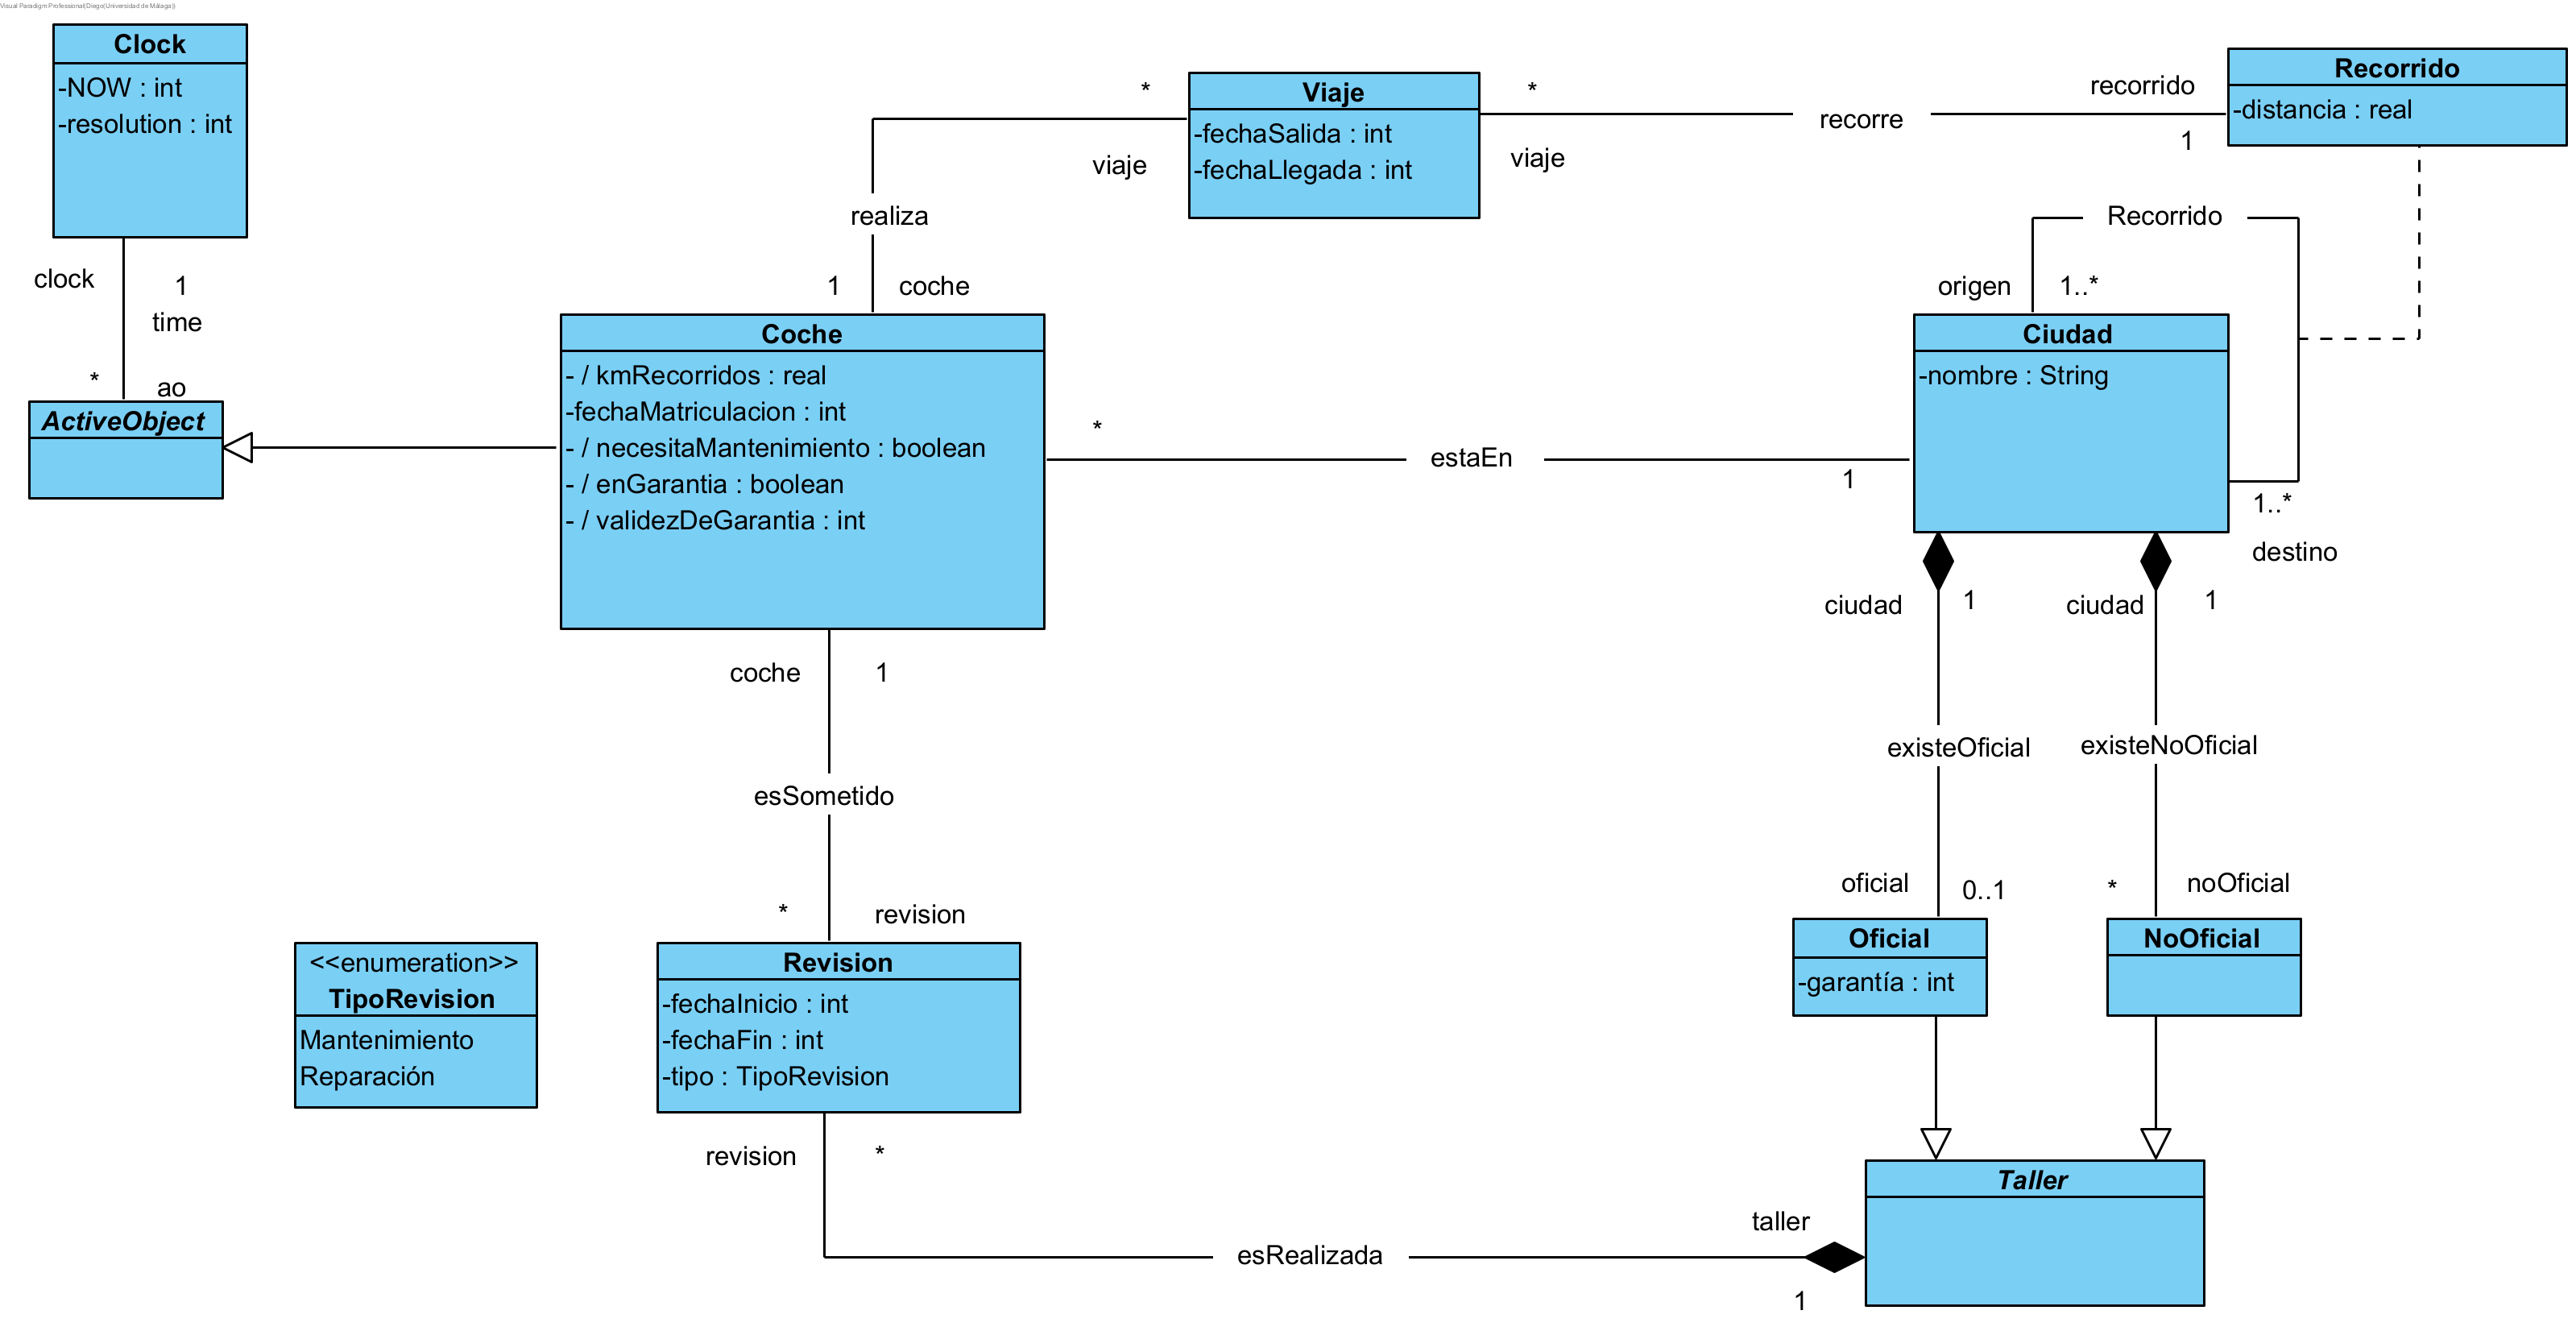
\includegraphics[width=1\linewidth]{diagramas/VPP_A.png}
     \caption{Diagrama del sistema de coches}
     \label{Diagrama del sistema de coches}
\end{figure}
\vspace{1.0 cm}

\subsection{Enumeraciones del Sistema}

\subsubsection{TipoRevision}
\textbf{Descripción}:  
Distingue entre los tipos de revisión a los que un coche se puede someter.
\begin{itemize}
    \item \textbf{Literales}:
    \begin{enumerate}
        \item \texttt{Mantenimiento}: Revisión obligatoria que cada coche necesita después de 4 años desde que se matriculó o después de 1 año desde la última revisión de mantenimiento que tuvo algún coche.
        \item \texttt{Reparación}: Revisión necesaria para la reparación de alguna avería en el coche.
    \end{enumerate}
\end{itemize}

\subsection{Clases del Sistema}

\subsubsection{Clock}
\textbf{Descripción}:  
Representa el elemento que lleva el conteo del instante actual en el que se encuentre el sistema y el valor los saltos que cada tick avanza en el tiempo. Se definió que cada unidad de tiempo equivale a un día y un año se representa con 100 días.
\begin{itemize}
    \item \textbf{Atributos}:
    \begin{itemize}
        \item \texttt{NOW: Integer}: Contador del tiempo registrado. Representa el instante actual en el que se encuentre el sistema.
        \item \texttt{resolution: Integer}: Valor de los saltos que hace el Clock en la llamada de cada tick.
    \end{itemize}
\end{itemize}

\subsubsection{ActiveObject} (Clase abstracta)
\textbf{Descripción}:  
Representa la clase padre de cualquier entidad del sistema que necesite un paso del tiempo para cambiar su estado. En este sistema solo \textbf{Coche} es una especificación de ActiveObject.

\subsubsection{Coche} (Subclase de ActiveObject)
\textbf{Descripción}:  
Representa un coche en el sistema. Cada coche puede realizar viajes entre ciudades y se someten a revisiones cuando lo requieran.
\begin{itemize}
    \item \textbf{Atributos}:
    \begin{itemize}
        \item \texttt{kmRecorridos: Real (derive)}: Atributo derivado que registra todos los kilómetros que el coche ha viajado entre ciudades como la suma de
        \textit{distancia} de cada \textit{recorrido} entre un par de ciudades.
        \item \texttt{fechaMatriculacion: Integer}: Marca el instante en el que el coche se ha registrado en el sistema.
        \item \texttt{necesitaMantenimiento: Boolean (derive)}: Atributo derivado que indica que el coche necesita ir a revisión \textit{Tipo: Mantenimiento} ya sea porque han pasado 4 años desde que se matriculó o pasó más de 1 año desde la última revisión de mantenimiento que tuvo.
        \item \texttt{enGarantia: Boolean (derive)}: Atributo derivado que indica que el coche tiene una garantía activa ya sea porque no han pasado 4 años desde que se matriculó o la \textit{validez de garantía} proporcionada por el \textit{Taller Oficial} donde se revisó sigue vigente. Un coche en garantía puede necesitar alguna revisión si las condiciones lo dictan.
        \item \texttt{validezDeGarantia: Integer (derive)}: Atributo derivado que indica los días por los que la garantía proporcionada por un \textit{Taller Oficial} está activa. En caso que un coche realice una revisión \textit{Tipo: Mantenimiento} en un \textit{Taller Oficial}, este recibirá la garantía comenzará a contar a la par que el año de garantía que el coche recibe por revisión de mantenimiento.
    \end{itemize}
\end{itemize}

\subsubsection{Revision}
\textbf{Descripción}: Representa la revisión que se le realizan a los coches en el sistema. Un coche puede realizar varias revisiones a lo largo del tiempo cuando esté obligado a hacerlo o lo necesite.
\begin{itemize}
    \item \textbf{Atributos}:
    \begin{itemize}
        \item \texttt{fechaInicio: Integer}: La fecha en la que se empezó la revisión del coche.
        \item \texttt{fechaFin: Integer}: La fecha en la que se finalizó la revisión del coche.
        \item \texttt{tipo: TipoRevisión}: Es el tipo de revisión que se le ha realizado al coche, que puede ser un mantenimiento o una reparación.
    \end{itemize}
\end{itemize}

\subsubsection{Taller} (Clase abstracta)
\textbf{Descripción}:  Representa un taller en el sistema y es la clase base para los diferentes tipos de taller. Las revisiones, independientemente del tipo, se realizan en un taller. 

\subsubsection{Oficial} (Subclase de \texttt{Taller})
\textbf{Descripción}:  Hereda de la clase Taller. Al realizar una revisión en este tipo de taller, el coche obtiene una garantía. Solo existe un taller oficial por ciudad.
\begin{itemize}
    \item \textbf{Atributos}:
    \begin{itemize}
        \item \texttt{garantía: Integer}: Duración de la garantía que ofrece el taller oficial.
    \end{itemize}
\end{itemize}

\subsubsection{No\texttt{\_}Oficial} (Subclase de \texttt{Taller})
\textbf{Descripción}:  Hereda de la clase Taller. A diferencia del taller oficial, si se realiza un mantenimiento en ese taller, no se da una garantía al coche. Pueden existir varios talleres no oficiales en una ciudad.

\subsubsection{Ciudad} (Clase abstracta)
\textbf{Descripción}: Representa una ciudad en el sistema en el que un coche viaja hacia esta.

\begin{itemize}
    \item \textbf{Atributos}:
    \begin{itemize}
        \item \texttt{nombre: String}: Nombre de la ciudad.
    \end{itemize}
\end{itemize}

\subsubsection{Recorrido} (Clase de Asociación entre Ciudad y Viaje)
\textbf{Descripción}: Representa el recorrido que se realiza durante un viaje para ir de una ciudad a otra en el sistema.

\begin{itemize}
    \item \textbf{Atributos}:
    \begin{itemize}
        \item \texttt{distancia: Double}: La distancia que hay entre la ciudad de origen y la de destino.
    \end{itemize}
\end{itemize}

\subsubsection{Viaje}
\textbf{Descripción}:  Representa los viajes en el sistema. 

\begin{itemize}
    \item \textbf{Atributos}:
    \begin{itemize}
        \item \texttt{fechaSalida: Integer}: La fecha de salida de la ciudad de origen del coche.
        \item \texttt{fechaLlegada: Integer}: La fecha de llegada a la ciudad de destino del coche.
    \end{itemize}
\end{itemize}

\vspace{2.0cm} % Espacio vertical de 2.0 cm

\subsection{Código USE}
\lstdefinestyle{useNormal}{
    basicstyle=\ttfamily\small,   % Estilo básico: letra monoespaciada pequeña
    keywordstyle=\color{blue},    % Color para palabras clave
    commentstyle=\color{green!50!black}, % Color para comentarios
    stringstyle=\color{red},      % Color para strings
    numberstyle=\tiny\color{gray}, % Color de los números de línea
    stepnumber=1,                 % Mostrar un número de línea en cada línea
    numbersep=10pt,               % Separación de los números del código
    tabsize=2,                    % Tamaño del tabulador
    showspaces=false,             % No mostrar espacios
    showstringspaces=false,       % No mostrar espacios en cadenas de texto
    breaklines=true,              % Ajustar líneas largas                  % Añadir un marco alrededor del código
}
\lstdefinestyle{useEspecifico}{
    basicstyle=\ttfamily\small,   % Estilo básico: letra monoespaciada pequeña
    backgroundcolor=\color{gray!10},  % Fondo gris claro
    keywordstyle=\color{blue},    % Color para palabras clave
    commentstyle=\color{green!50!black}, % Color para comentarios
    stringstyle=\color{red},      % Color para strings
    numberstyle=\tiny\color{gray}, % Color de los números de línea
    stepnumber=1,                 % Mostrar un número de línea en cada línea
    numbersep=10pt,               % Separación de los números del código
    tabsize=4,                    % Tamaño del tabulador
    showspaces=false,             % No mostrar espacios
    showstringspaces=false,       % No mostrar espacios en cadenas de texto
    breaklines=true,              % Ajustar líneas largas
    frame=single                  % Añadir un marco alrededor del código
}
A continuación mostraremos todo el código desarrollado con el lenguaje USE, están divididos en varios sectores:


\begin{itemize}
    \item \textbf{‘Enumeraciones’}: Representa los distintos valores que un atributo puede tomar en un momento dado en sistema.
    \item \textbf{‘Clases’}: Representa todas las entidades del sistema.
    \item \textbf{‘Relaciones’}: Representa las interacciones existentes entre entidades.
    \item \textbf{‘Invariantes’}: Representa todas las restricciones del sistema a manejar.
\end{itemize}
Todo el código suministrado ha sido realizado en VSCode y
todas las secciones están separadas por sus respectivos títulos tabulados en mayúsculas.
\vspace{1cm}
\begin{lstlisting}[style = useNormal,language=SQL, caption={Modelo de Sistema de Coches en USE}] 

ENUMERACIONES

enum TipoRevision{Mantenimiento, Reparacion}

CLASES 

class Clock
attributes
    NOW : Integer --init = 0            
    resolution : Integer --init = 1
end

abstract class ActiveObject
end

class Coche < ActiveObject
attributes
    kmRecorridos : Real derive :        
        self.viaje.recorrido -> collect(dist | dist.distancia) -> sum()
        
    fechaMatriculacion : Integer            

    necesitaMantenimiento : Boolean derive : 
        if self.clock.NOW  - fechaMatriculacion < 400 
            then
                false
            else
                let ultimaRevision : Revision = self.revision -> select(rev | rev.tipo = TipoRevision::Mantenimiento) -> sortedBy(r | r.fechaInicio) -> last() in
                if ultimaRevision <> null
                then
                    (self.clock.NOW - ultimaRevision.fechaFin) > 100
                else
                    true
                endif
        endif

    enGarantia : Boolean derive :             
        ((self.clock.NOW  - fechaMatriculacion) < 400) or
        (validezDeGarantia > 0)

    validezDeGarantia : Integer derive :   
        if (self.clock.NOW - fechaMatriculacion) < 400 
            then 
                400 - (self.clock.NOW  - fechaMatriculacion) 
            else
                let revisionesOficiales : OrderedSet(Revision) = self.revision -> select(rev | rev.taller.oclIsKindOf(Oficial)) -> sortedBy(rev | rev.fechaInicio) in
                    if (self.clock.NOW - (revisionesOficiales -> last()).fechaFin) < (revisionesOficiales -> last()).taller.oclAsType(Oficial).garantia
                        then
                            (revisionesOficiales -> last()).taller.oclAsType(Oficial).garantia - (self.clock.NOW - (revisionesOficiales -> last()).fechaFin)
                        else 
                            0
                    endif          
        endif 
end 

class Viaje
attributes
    fechaSalida : Integer                     
    fechaLlegada : Integer 
end

class Revision
attributes
    tipo : TipoRevision                   
    fechaInicio : Integer                     
    fechaFin : Integer                      
end

abstract class Taller                        
end

class Oficial < Taller                      
    garantia : Integer                      
end

class NoOficial < Taller                     
end 

class Ciudad
attributes
    nombre : String                          
end


CLASE DE ASOCIACION

associationclass Recorrido between
    Ciudad [1] role destino Ciudad [1] role origen
attributes
    distancia : Real                    
end 


RELACIONES

association time between
Clock [1] role clock
ActiveObject [*] role ao
end

association realiza between
Coche [1] role coche
Viaje [*] role viaje
end

association recorre between
Viaje [*] role viaje
Recorrido [1] role recorrido
end

association estaEn between
Coche [*] role coche
Ciudad [1] role ciudad
end

association esSometido between
Coche [1] role coche
Revision [*] role revision
end

composition esRealizada between
Taller [1] role taller
Revision [*] role revision
end

composition existeOficial between
Ciudad [1] role ciudad
Oficial [0..1] role oficial
end

composition existeNoOficial between
Ciudad [1] role ciudad
NoOficial [*] role  NoOficial
end



\end{lstlisting}
\vspace{1cm}
\subsection{Diagrama de Clases en USE}
La herramienta USE nos permite llevar a cabo un diagrama de clases, el cual se muestra a continuación:
\begin{figure}[H]
     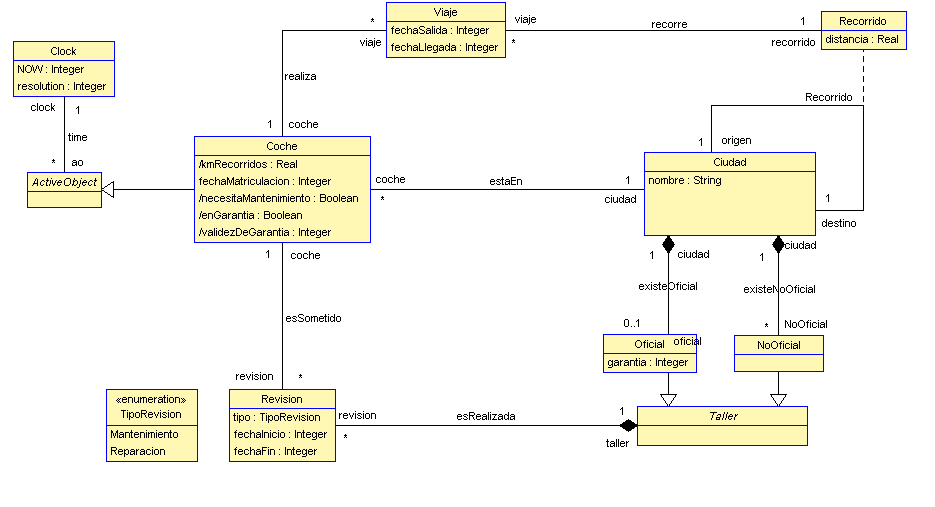
\includegraphics[width=1\linewidth]{diagramas/USE_A.png}
     \caption{Diagrama del sistema de coches en USE}
     \label{Diagrama del sistema de coches en USE}
\end{figure}
\vspace{1.0cm}

Todas las relaciones entre las entidades del modelo tienen su significado y están definidas de la siguiente manera:
\begin{itemize}
\item \textbf{esSometido (Coche-Revisión)}:  Esta relación indica que cada coche en el sistema puede estar asociado a múltiples revisiones a lo largo de su vida útil. Cada revisión se registra cuando el coche necesita mantenimiento o reparación.
  
\item \textbf{realiza (Coche-Viaje))}: Relación que representa el hecho de que un coche puede realizar varios viajes. Un viaje es un desplazamiento que inicia en una ciudad y concluye en otra, y se registra en el sistema para hacer seguimiento del historial de movimientos del coche.

\item \textbf{estaEn (Coche-Ciudad)}: Esta relación representa la ubicación actual del coche en una ciudad. Cada coche estará siempre en una ciudad específica, ya sea de origen o destino de algún viaje.

\item \textbf{esRealizada (Revisión-Taller)}: Define que toda revisión de un coche debe realizarse en un taller. Esto significa que las revisiones de mantenimiento y reparación se registran con el taller en el que se realizan.

\item \textbf{existeOficial (Oficial-Ciudad)}: Relación que establece la existencia de un único taller oficial en cada ciudad. El taller oficial ofrece revisiones con garantía, lo cual beneficia a los coches que pasan por él.

\item \textbf{existeNoOficial (NoOficial-Ciudad)}: Representa la existencia de uno o varios talleres no oficiales en cada ciudad. Estos talleres pueden realizar revisiones de mantenimiento y reparación, pero no otorgan garantía a los coches.

\item \textbf{Recorrido (Ciudad-Ciudad)}: Relación de asociación entre dos ciudades, que define la distancia entre ellas. Esto permite modelar la distancia que un coche debe recorrer al viajar de una ciudad a otra.

\item \textbf{time (Clock-ActiveObject)}: Esta relación conecta la instancia única de Clock con cada objeto activo (ActiveObject) del sistema, como los coches. A través de esta relación, el sistema puede realizar el seguimiento del paso del tiempo y cómo afecta a cada coche o entidad que depende del tiempo para su funcionamiento o estado.
\end{itemize}

\subsection{Invariantes y .SOIL}
Para poder comprobar las restricciones de nuestro sistema, primero es necesario definir las reglas que aseguran su correcto funcionamiento. Las restricciones o invariantes que se han definido son las siguientes:

\begin{itemize}
    \item \textbf{1.}: Cada ciudad debe tener una distancia minima de 5 km para cada recorrido.
    \begin{lstlisting}[style = useEspecifico,language=SQL]
    context Recorrido
      inv minimo5Km :
      self . distancia >= 5
    \end{lstlisting}
    Asegura que cada recorrido tenga una distancia mínima de 5 km. Esto podría ser para evitar registrar viajes demasiado cortos que no sean relevantes en el contexto del sistema. Además hemos decidido que si hay un recorrido entre una misma ciudad dicho recorrido debe ser mayor a 5 kilometros también.
    
    \item \textbf{2.}: Cada coche debe de pasar revision despues de matricularse y no antes.
    \begin{lstlisting}[style = useEspecifico,language=SQL]
   context Coche
     inv revisionDespuesdeMatriculacion:
     self.revision -> forAll(rev | rev.fechaInicio > self.fechaMatriculacion)
    \end{lstlisting}
    Tiene que pasar obligatoriamente después porque antes de la fecha de matriculación no existe el dicho coche en nuestro modelo.
    Compara la fecha de matriculación del coche con la fecha de inicio de cada revisión asociada a él, y verifica que todas las revisiones cumplan con esta condición. 
    
    \item \textbf{3.}: Todos los coches han de ser revisados como máximo en un momento dado.
    \begin{lstlisting}[style = useEspecifico,language=SQL]
    inv revisadoUnaVez:
    self.revision -> forAll(rev1, rev2 | not(rev1 <> rev2) or rev1.fechaInicio <> rev2.fechaInicio and (rev1.fechaInicio >= rev2.fechaFin or rev2.fechaInicio >= rev1.fechaFin))
    \end{lstlisting}
    Restringe a cada coche a ser revisado solo una vez en un tiempo dado, evitando revisiones superpuestas en el tiempo.
    Lo que hace es revisar las fechas de inicio y fin de cada revisión para asegurarse de que ninguna de ellas se superponga.
    
    \item \textbf{4.}: Si un coche esta en revision, debe de estar en la misma ciudad que el taller.
    \begin{lstlisting}[style = useEspecifico,language=SQL]
  context Revision
    inv mismaCiudadqueTallerEnRevision:
    ((self.coche.clock -> asOrderedSet() -> first()).NOW - self.fechaFin) < 0 implies
    (self.taller.oclIsKindOf(Oficial) and self.taller.oclAsType(Oficial).ciudad = self.coche.ciudad) or (self.taller.oclIsKindOf(No_Oficial) and self.taller.oclAsType(No_Oficial).ciudad = self.coche.ciudad)
    \end{lstlisting}
    Asegura que un coche en revisión se encuentre en la misma ciudad que el taller donde se realiza la revisión. Esto garantiza que el coche y el taller están físicamente en el mismo lugar cuando se realiza el mantenimiento.
    Verifica la ciudad asociada al taller y la compara con la ciudad en la que se encuentra el coche en ese momento.
    
    \item \textbf{5.}: Un coche tiene que estar o viajando o en una ciudad.
    \begin{lstlisting}[style = useEspecifico,language=SQL]
  context Viaje
    inv viajandoOenCiudad:
    let currentTime : Integer = self.coche.clock.NOW in
    (currentTime - self.fechaLlegada) < 0 implies
    self.coche.ciudad.oclIsUndefined() -- and self.coche.estaEn->notEmpty()
    \end{lstlisting}
    Asegura que un coche se encuentre en una ciudad o esté realizando un viaje, pero no ambas cosas a la vez. Esto previene conflictos de ubicación, indicando que un coche en movimiento no está en una ciudad específica hasta que llegue a su destino.
    Evalúa si el coche está en un viaje actualmente (determinando que su fecha de llegada es futura) y, si es así, asegura que el coche no tenga una ciudad asignada hasta que termine el viaje.
    
    \item \textbf{6.}: Un coche después de su viaje tiene que encontrarse en su ciudad destino.
    \begin{lstlisting}[style = useEspecifico,language=SQL]
  context Coche
    inv enCiudadDestino:
    let ultimoViaje : Viaje = self.viaje -> asOrderedSet() -> sortedBy(fechaLlegada) -> last() in
    ultimoViaje.recorrido.destino = self.ciudad
    \end{lstlisting}
    Establece que, al finalizar un viaje, el coche se encuentra en la ciudad de destino del recorrido, asegurando que los viajes finalicen en el lugar esperado.
    Verifica la última ciudad de destino registrada y la compara con la ubicación actual del coche, garantizando coherencia en la posición final.
    
    \item \textbf{7.}: No pueden haber dos viajes solapados.
    \begin{lstlisting}[style = useEspecifico,language=SQL]
  context Coche
    inv viajeUnico:
    self.viaje -> forAll(v1,v2 | not(v1 <> v2) or v1.fechaSalida <> v2.fechaSalida and (v1.fechaLlegada <= v2.fechaSalida or v2.fechaLlegada <= v1.fechaSalida))
    \end{lstlisting}
    Impide que un coche tenga dos viajes concurrentes, asegurando que un coche solo pueda realizar un viaje a la vez.
    Revisa las fechas de inicio y fin de cada viaje asociado al coche y se asegura de que no existan superposiciones, es decir, que los períodos de cada viaje sean únicos.
    
    \item \textbf{8.}: Un coche debe de empezar el siguiente viaje en la ciudad destino del anterior.
    \begin{lstlisting}[style = useEspecifico,language=SQL]
    inv destinoComoOrigen:
    let viajesOrdenados : OrderedSet(Viaje)  = self.viaje -> sortedBy(v | v.fechaSalida) in 
    viajesOrdenados -> forAll(v1, v2 | viajesOrdenados->indexOf(v1) = viajesOrdenados->indexOf(v2) + 1 implies v1.recorrido.destino = v2.recorrido.origen)
    \end{lstlisting}
    Asegura que el siguiente viaje de un coche comience en la ciudad de destino de su viaje anterior, lo que garantiza una secuencia lógica de viajes.
    Para lograr esto, ordena los viajes en secuencia temporal y verifica que cada destino sea el punto de partida del siguiente viaje.
    
    \item \textbf{9.}: Una ciudad tiene que tener un recorrido con otra ciudad de manera obligatoria
    \begin{lstlisting}[style = useEspecifico,language=SQL]
  context Ciudad
    inv hayRecorridos:
    self.origen -> notEmpty() and self.destino -> notEmpty()
    \end{lstlisting}
    Asegura que cada ciudad tenga recorridos que la conecten con otras ciudades, promoviendo la conectividad en el sistema y evitando que existan ciudades aisladas.
    Verifica que existan recorridos que incluyan la ciudad como punto de partida o de llegada.
    
    \item \textbf{10.}: Un coche debe de estar en la ciudad destino de su último viaje antes de iniciar un viaje.
    \begin{lstlisting}[style = useEspecifico,language=SQL]
  context Coche
    inv empiezaViajeEnDestino:
    (self.viaje -> asOrderedSet() -> sortedBy(fechaSalida) -> last()).recorrido.destino = self.ciudad
    \end{lstlisting}
     Define que un coche debe estar en la ciudad de destino de su último viaje antes de comenzar otro viaje, garantizando consistencia en la ubicación del coche entre viajes.
     Ordena los viajes de un coche en secuencia y compara el destino del último viaje con el origen del siguiente, asegurando que el coche no "salte" de una ciudad a otra sin haber llegado previamente a esa ubicación. Esto mantiene la coherencia en los desplazamientos del coche.
     
    \item \textbf{11.}: Cada coche debe de pasar revision despues de matricularse y no antes.
    \begin{lstlisting}[style = useEspecifico,language=SQL]
    inv viajeDespuesdeMatriculacion:
    self.viaje -> forAll(viaje | viaje.fechaSalida > self.fechaMatriculacion)    
    \end{lstlisting}
    Restringe a los coches a realizar viajes solo después de su fecha de matriculación, lo que previene errores lógicos de viajes previos al registro oficial del vehículo.
    Compara la fecha de matriculación con la fecha de salida de cada viaje y asegura que todos los viajes comiencen después de dicha fecha.
    
    \item \textbf{12.}: Un coche no debe poder comenzar un viaje con la alerta de mantenimiento en true.
    \begin{lstlisting}[style = useEspecifico,language=SQL]
    inv noViajeEnMantenimiento:
    self.necesitaMantenimiento implies self.viaje -> forAll(v | v.fechaLlegada < self.clock.NOW)   
    \end{lstlisting}
    Asegura que un coche con alerta de mantenimiento no inicie ningún viaje, promoviendo la seguridad y mantenimiento adecuado.
    Esto se logra comprobando que si necesitaMantenimiento es true, todos los viajes del coche ya hayan finalizado antes del tiempo actual 
    
    \item \textbf{13.}: Un viaje no puede tener una fecha de inicio superior a su fecha de llegada.
    \begin{lstlisting}[style = useEspecifico,language=SQL]
context Viaje
    inv fechaViajeBienDefinida:
    self.fechaLlegada >= self.fechaSalida  
    \end{lstlisting}
    Asegura que la fecha de salida de un viaje sea anterior o igual a su fecha de llegada, previniendo datos inconsistentes en los registros de viaje.
\end{itemize}

\subsection{Diagramas de objetos para cada restricción}
A partir de aqui podemos desarrollar los archivos de prueba que respaldaran el funcionamiento de nuestro sistema. Vamos a comprobar restricción por restricción, comprobando cada caso con un ejemplo y un contraejemplo.

Hemos considerado, por las peticiones de concisión y brevedad, que la inclusión del código soil de cada uno de los modelos de objetos que comprueban invariantes y derivados enturbia y  entorpece la lectura y comprensión del documento. A continuación se muestran los diagramas resultantes de dichos códigos, junto a sus comprobaciones. Los códigos fuente se han adjuntado con la entrega.

\subsubsection{Invariante 1: mínimo5Km}

\vspace{1.0 cm}
\begin{figure}[H]
     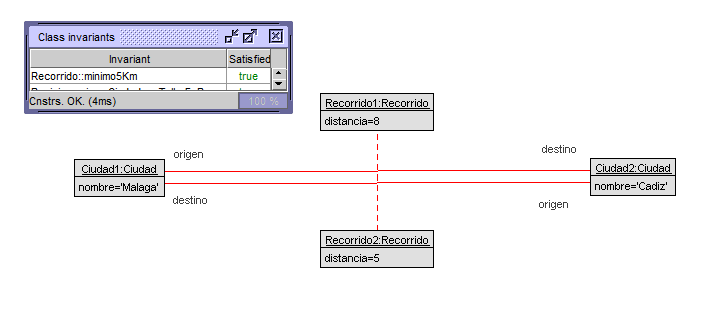
\includegraphics[width=1\linewidth]{Soils/1_v2.png}
     \caption{Diagrama de objetos para la invariante al cumplirse}
     \label{Diagrama del sistema de aviacion}
\end{figure}

\begin{figure}[H]
     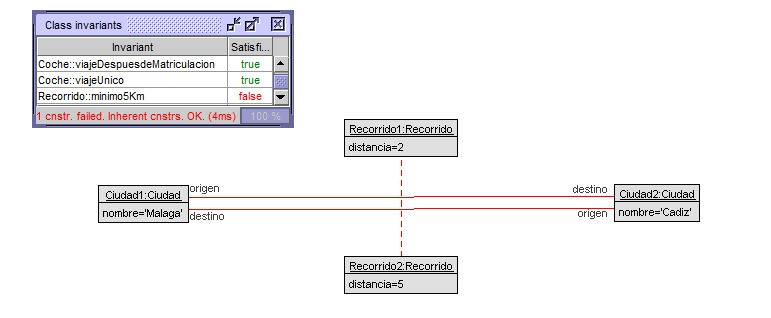
\includegraphics[width=1\linewidth]{Soils/1.jpg}
     \caption{Diagrama de objetos para la invariante al incumplirse}
     \label{Diagrama del sistema de aviacion}
\end{figure}

La invariante 1 garantiza que cada recorrido entre ciudades tenga una distancia mínima de 5 km. Se considera cumplida si la distancia del recorrido es igual o superior a 5 km, y no cumplida si el recorrido es menor a esa distancia.

\subsubsection{Invariante 2: revisionDespuesdeMatriculacion}
\begin{figure}[H]
    \centering
     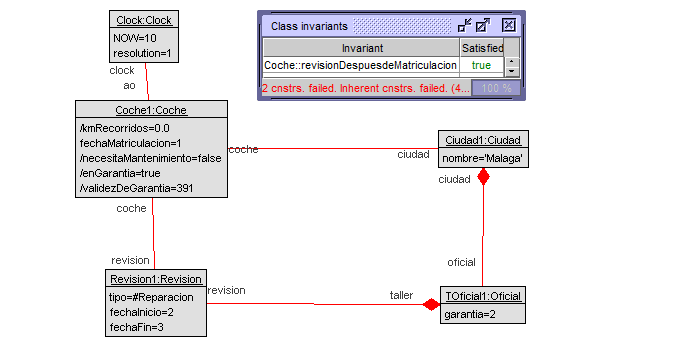
\includegraphics[width=0.75\linewidth]{Soils/2_v2.png}
     \caption{Diagrama de objetos para la invariante al cumplirse}
     \label{Diagrama del sistema de aviacion}
\end{figure}

\begin{figure}[H]
    \centering
    \begin{minipage}{0.49\textwidth}
        \centering
        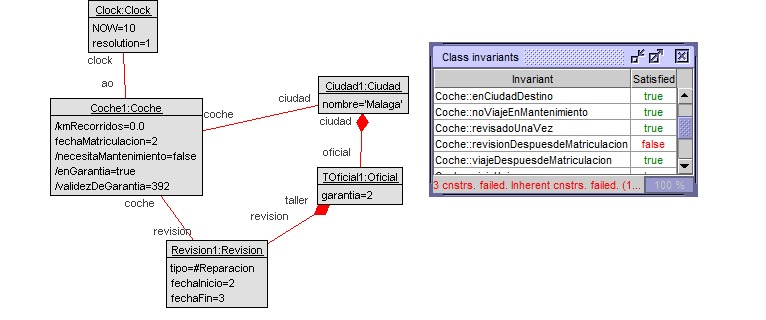
\includegraphics[width=1\linewidth]{Soils/2.jpg}
        \label{fig:diagrama1}
    \end{minipage}
    \hfill
    \begin{minipage}{0.49\textwidth}
        \centering
        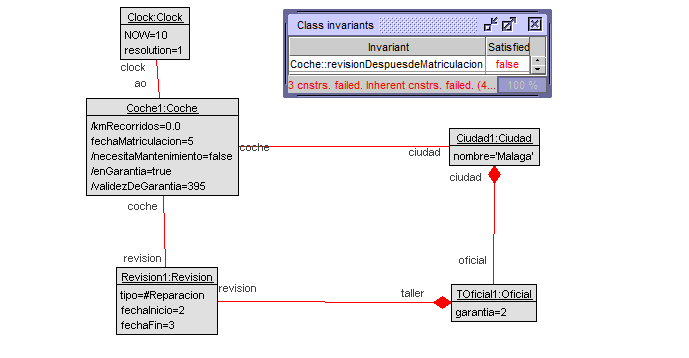
\includegraphics[width=1\linewidth]{Soils/2_v3.png}
        \label{fig:diagrama2}
    \end{minipage}
    \caption{Diagramas de objetos para la invariante al incumplirse}
    \label{fig:diagrama_invariante}
\end{figure}


La invariante 2 garantiza que cada coche pase su revisión después de la matriculación. Se considera cumplida si las revisiones ocurren después de esta fecha y no cumplida si la revisión se realiza el mismo día o antes de la matriculación.

\subsubsection{Invariante 3: revisadoUnaVez}
    \begin{figure}[H]
         \centering
         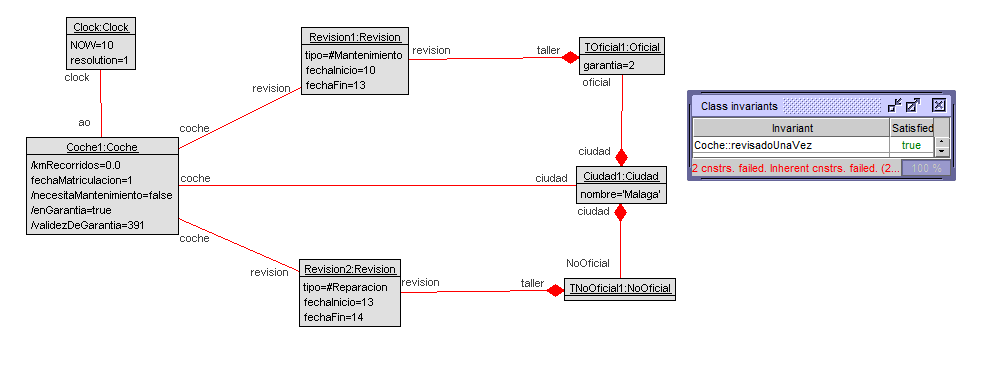
\includegraphics[width=1\linewidth]{Soils/3.png}
         \caption{Diagrama de objetos para la invariante al cumplirse}
         \label{Diagrama_cumplimiento}
    \end{figure}

    
   \begin{figure}[H]
    \centering
    \begin{minipage}{0.49\textwidth}
        \centering
        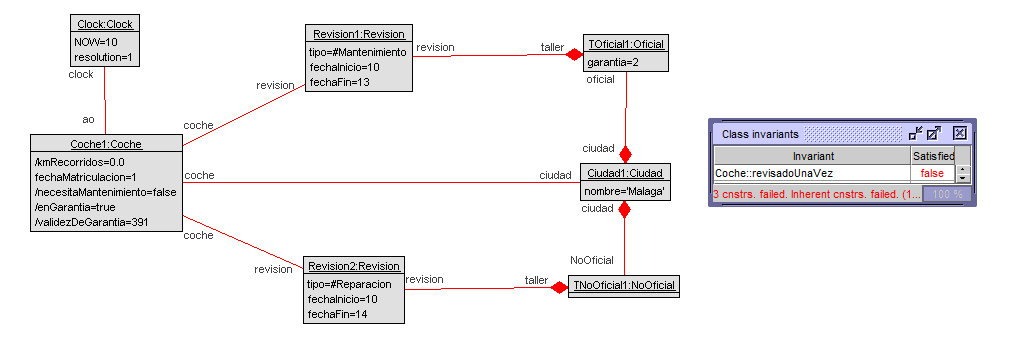
\includegraphics[width=\linewidth]{Soils/3_v2.png}
        \label{fig:diagrama1}
    \end{minipage}
    \hfill
    \begin{minipage}{0.49\textwidth}
        \centering
        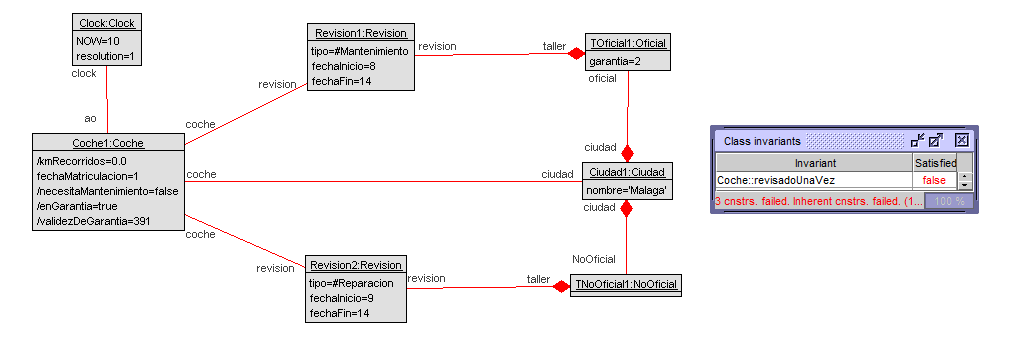
\includegraphics[width=\linewidth]{Soils/3_v3.png}
        \label{fig:diagrama2}
    \end{minipage}
    \hfill
        \centering
        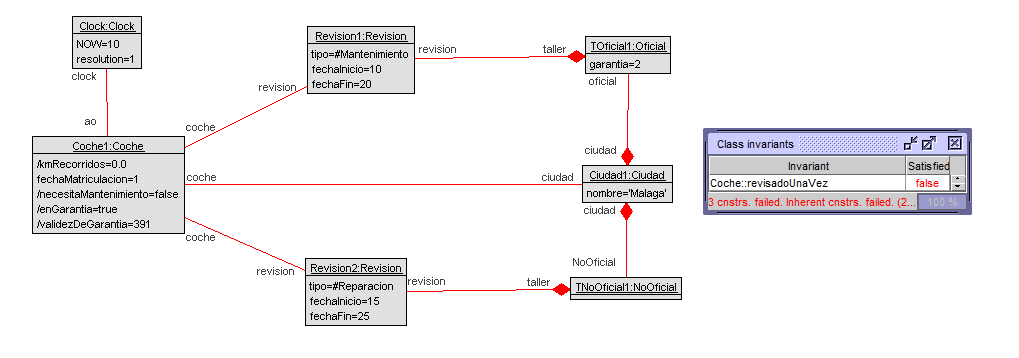
\includegraphics[width=0.7\linewidth]{Soils/3_v4.png}
        \label{fig:diagrama3}
    \caption{Diagramas de objetos para la invariante al incumplirse}
    \label{fig:Diagrama_incumplimiento}
\end{figure}


La invariante 3 garantiza que cada coche sea revisado como máximo en un único momento dado. Se considera cumplida si no existen revisiones que se solapen, ya sea por fecha de inicio, fecha de finalización o si una revisión empieza antes de que termine otra. No se cumple cuando dos revisiones a un coche coinciden en sus fechas de inicio, finalización o si una comienza antes de que termine la otra.

\subsubsection{Invariante 4: mismaCiudadqueTallerEnRevision}
    \begin{figure}[H]
         \centering
         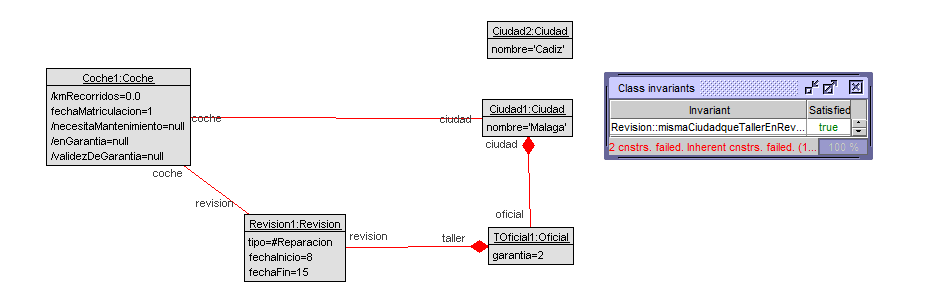
\includegraphics[width=1\linewidth]{Soils/4.png}
         \caption{Diagrama de objetos para la invariante al cumplirse}
         \label{Diagrama_cumplimiento}
    \end{figure}

    
 \begin{figure}[H]
    \centering
    \begin{minipage}{0.49\textwidth}
        \centering
        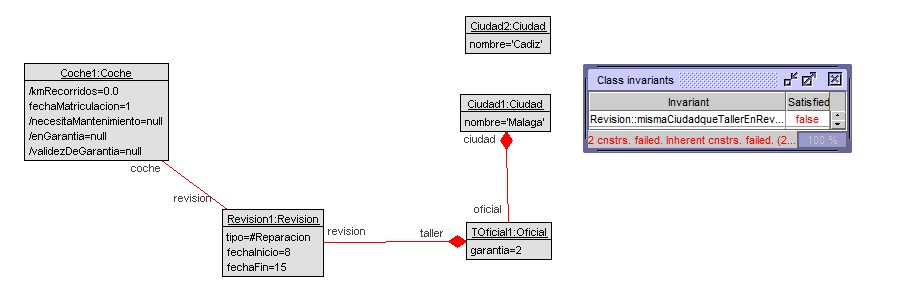
\includegraphics[width=1\linewidth]{Soils/4_v2.png}
        \label{fig:diagrama1}
    \end{minipage}
    \hfill
    \begin{minipage}{0.49\textwidth}
        \centering
        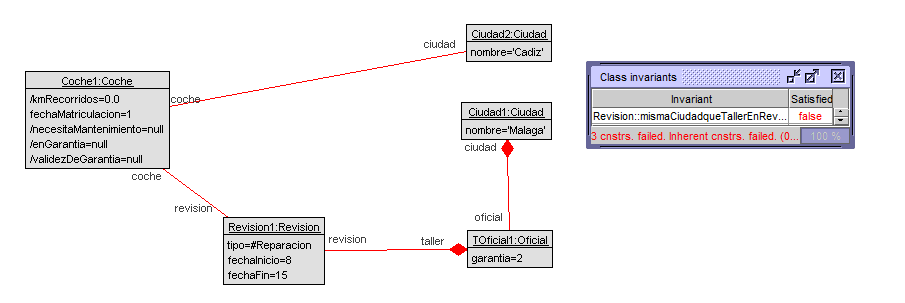
\includegraphics[width=1\linewidth]{Soils/4_v3png.png}
        \label{fig:diagrama2}
    \end{minipage}
    \caption{Diagramas de objetos para la invariante al incumplirse}
    \label{fig:diagrama_invariante}
\end{figure}

La invariante 4 establece que un coche en revisión debe encontrarse en la misma ciudad que el taller donde se realiza la revisión. Se considera cumplida si el coche está en la misma ciudad que el taller. No se cumple cuando el coche no está en ninguna ciudad o si se encuentra en una ciudad distinta a la del taller.

\subsubsection{Invariante 5: viajandoOenCiudad}

\vspace{1.0 cm}
\begin{figure}[H]
     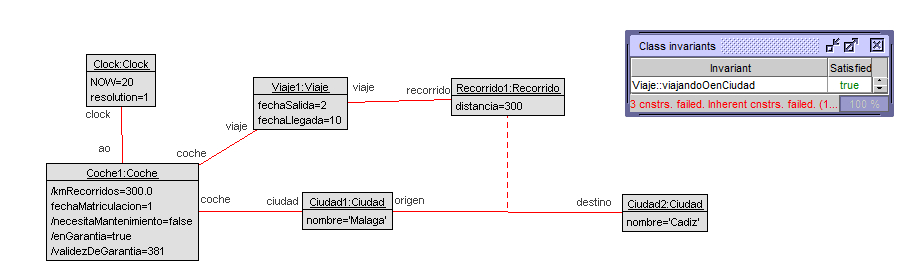
\includegraphics[width=1\linewidth]{Soils/5.png}
     \caption{Diagrama de objetos para la invariante al cumplirse}
     \label{Diagrama del sistema de aviacion}
\end{figure}

\begin{figure}[H]
     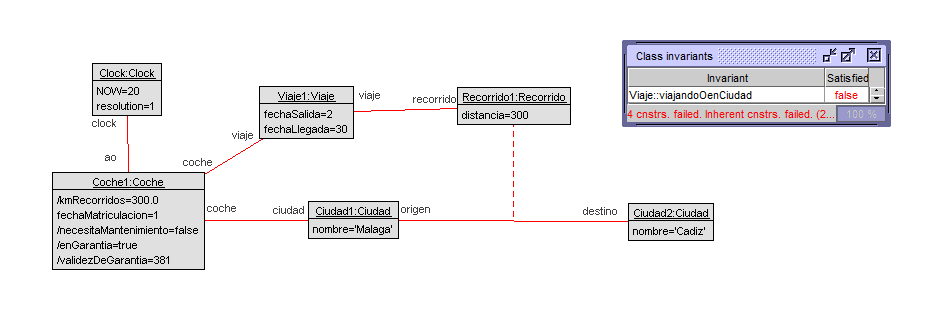
\includegraphics[width=1\linewidth]{Soils/5_v2.png}
     \caption{Diagrama de objetos para la invariante al incumplirse}
     \label{Diagrama del sistema de aviacion}
\end{figure}

La invariante 5 establece que un coche debe estar exclusivamente viajando o en una ciudad en un momento dado. Se considera cumplida si el coche se encuentra en una de estas dos condiciones. No se cumple cuando el coche está simultáneamente viajando y en una ciudad.

\subsubsection{Invariante 6: enCiudadDestino}
    \begin{figure}[H]
         \centering
         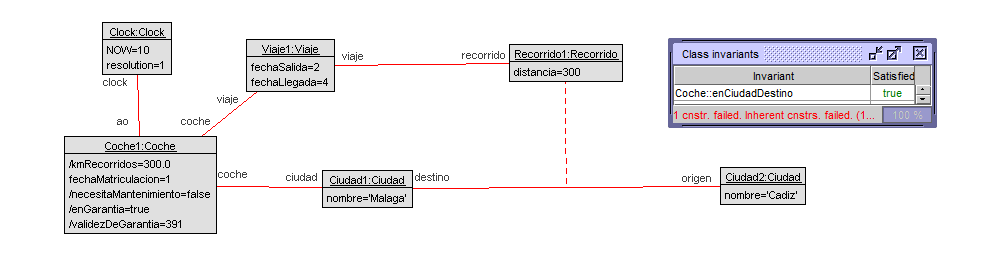
\includegraphics[width=1\linewidth]{Soils/6.png}
         \caption{Diagrama de objetos para la invariante al cumplirse}
         \label{Diagrama_cumplimiento}
    \end{figure}

    
 \begin{figure}[H]
    \centering
    \begin{minipage}{0.49\textwidth}
        \centering
        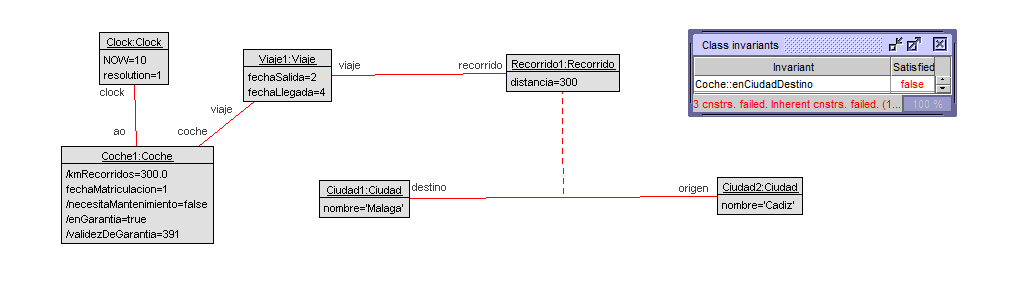
\includegraphics[width=1\linewidth]{Soils/6_v2.png}
        \label{fig:diagrama1}
    \end{minipage}
    \hfill
    \begin{minipage}{0.49\textwidth}
        \centering
        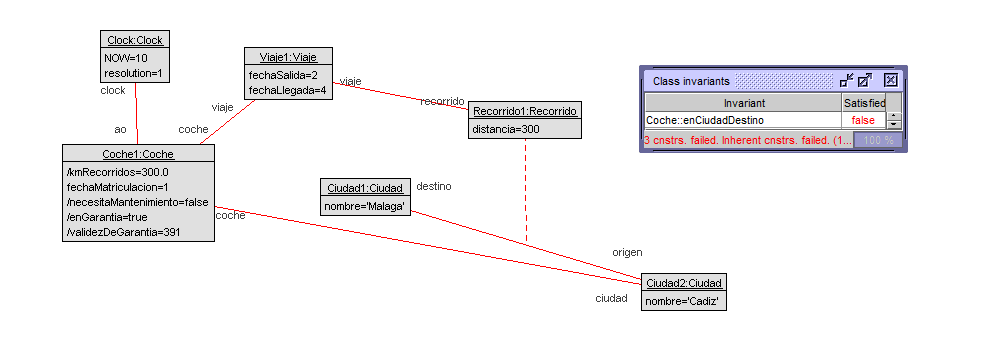
\includegraphics[width=1\linewidth]{Soils/6_v3.png}
        \label{fig:diagrama2}
    \end{minipage}
    \caption{Diagramas de objetos para la invariante al incumplirse}
    \label{fig:diagrama_invariante}
\end{figure}

La invariante 6 establece que un coche, después de completar su viaje, debe encontrarse en su ciudad destino. Se cumple cuando el coche está en la ciudad de destino al finalizar el viaje. No se cumple si, al finalizar el viaje, el coche no se encuentra en ninguna ciudad o si está en una ciudad diferente a la de destino.

\subsubsection{Invariante 7: viajeUnico}
    \begin{figure}[H]
         \centering
         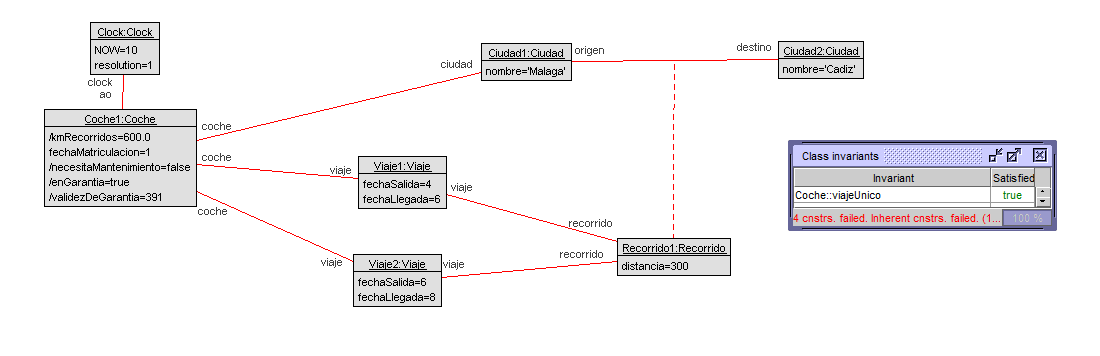
\includegraphics[width=1\linewidth]{Soils/7.png}
         \caption{Diagrama de objetos para la invariante al cumplirse}
         \label{Diagrama_cumplimiento}
    \end{figure}

  \begin{figure}[H]
    \centering
    \begin{minipage}{0.49\textwidth}
        \centering
        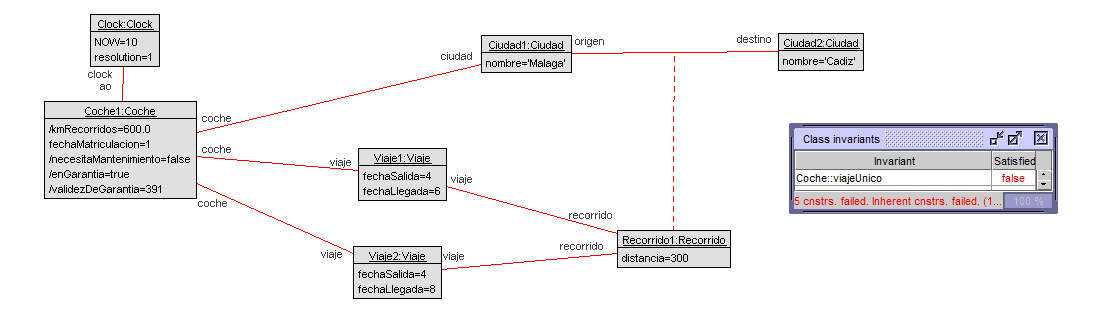
\includegraphics[width=\linewidth]{Soils/7_v2.png}
        \label{fig:diagrama1}
    \end{minipage}
    \hfill
    \begin{minipage}{0.49\textwidth}
        \centering
        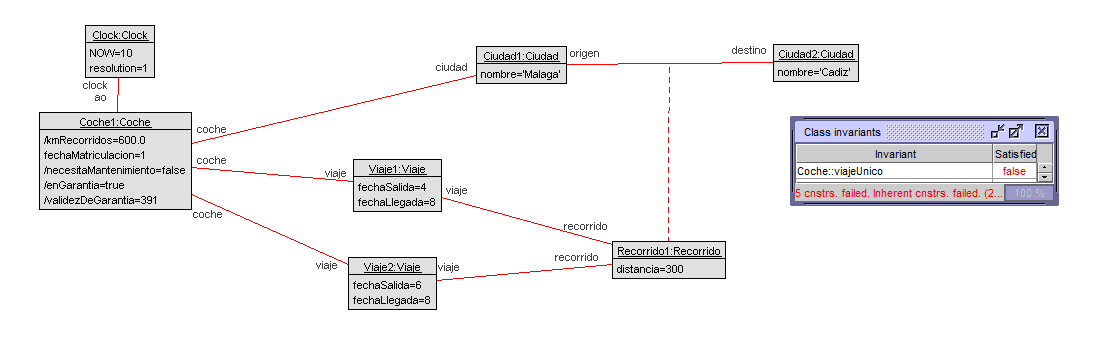
\includegraphics[width=\linewidth]{Soils/7_v3.png}
        \label{fig:diagrama2}
    \end{minipage}
    \hfill
        \centering
        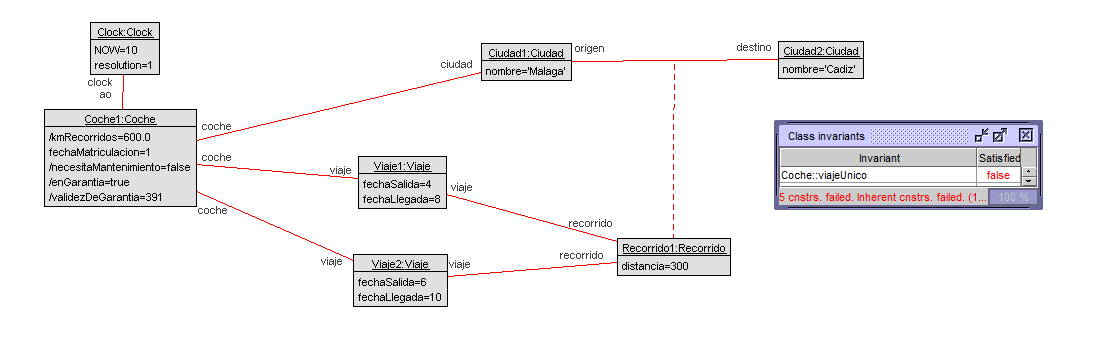
\includegraphics[width=0.7\linewidth]{Soils/7_v4.png}
        \label{fig:diagrama3}
    \caption{Diagramas de objetos para la invariante al incumplirse}
    \label{fig:Diagrama_incumplimiento}
\end{figure}

La invariante 7 establece que no pueden existir dos viajes solapados. Se considera cumplida cuando las fechas de inicio y finalización de los viajes no coinciden. No se cumple si las fechas de inicio o finalización de dos viajes coinciden o si un viaje comienza antes de que termine otro viaje del mismo coche.

\subsubsection{Invariante 8: destinoComoOrigen}

\vspace{1.0 cm}
\begin{figure}[H]
     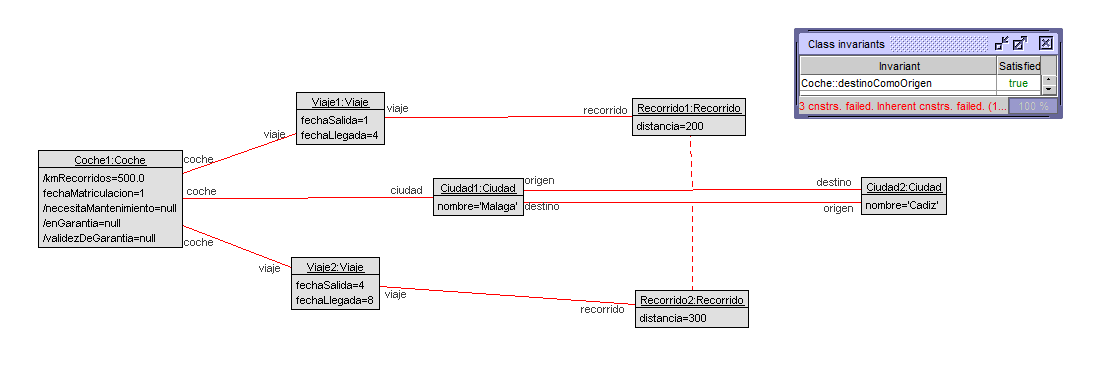
\includegraphics[width=1\linewidth]{Soils/8.png}
     \caption{Diagrama de objetos para la invariante al cumplirse}
     \label{Diagrama del sistema de aviacion}
\end{figure}

\begin{figure}[H]
     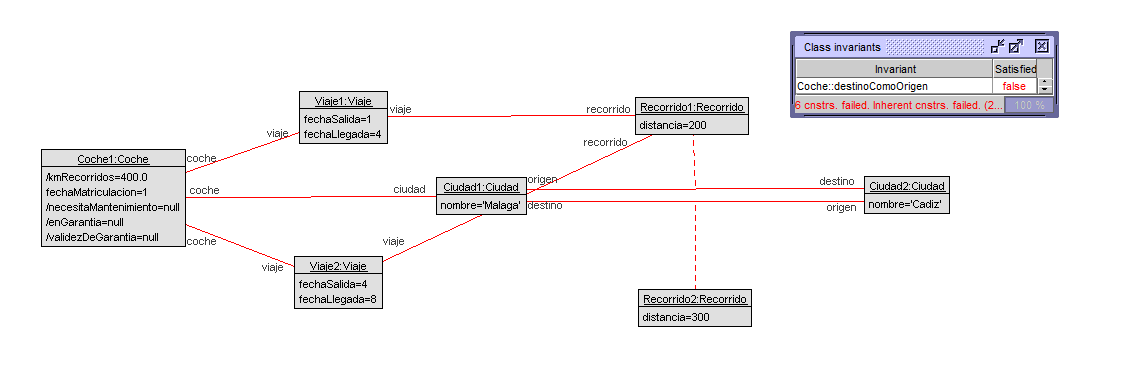
\includegraphics[width=1\linewidth]{Soils/8_v2.png}
     \caption{Diagrama de objetos para la invariante al incumplirse}
     \label{Diagrama del sistema de aviacion}
\end{figure}

La invariante 8 exige que un coche comience su siguiente viaje en la ciudad de destino del anterior. Se cumple cuando el coche inicia su viaje en la ciudad de destino del viaje anterior. No se cumple si el coche comienza el siguiente viaje en una ciudad diferente.

\subsubsection{Invariante 9: hayRecorridos}
    \begin{figure}[H]
         \centering
         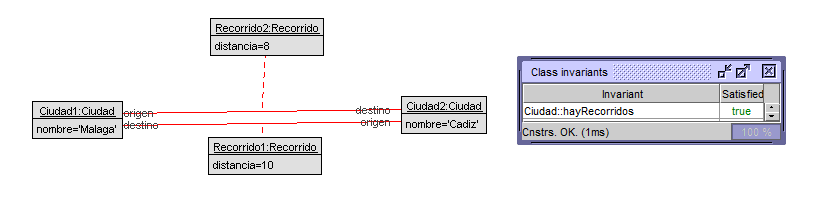
\includegraphics[width=1\linewidth]{Soils/9.png}
         \caption{Diagrama de objetos para la invariante al cumplirse}
         \label{Diagrama_cumplimiento}
    \end{figure}

  \begin{figure}[H]
    \centering
    \begin{minipage}{0.49\textwidth}
        \centering
        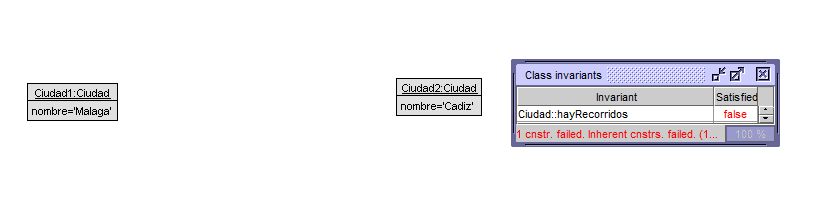
\includegraphics[width=\linewidth]{Soils/9_v2.png}
        \label{fig:diagrama1}
    \end{minipage}
    \hfill
    \begin{minipage}{0.49\textwidth}
        \centering
        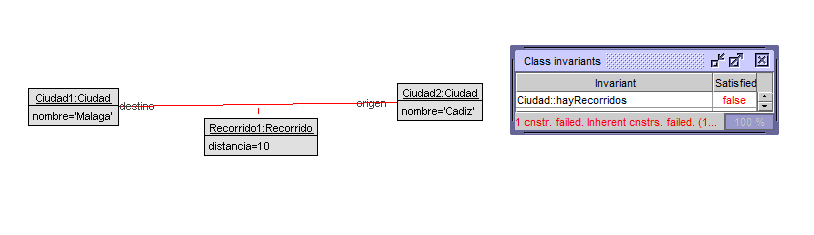
\includegraphics[width=\linewidth]{Soils/9_v3.png}
        \label{fig:diagrama2}
    \end{minipage}
    \hfill
        \centering
        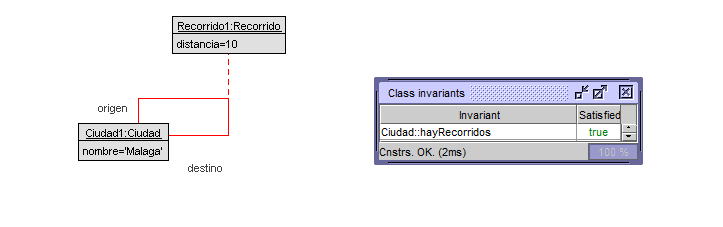
\includegraphics[width=0.7\linewidth]{Soils/9_v4.png}
        \label{fig:diagrama3}
    \caption{Diagramas de objetos para la invariante al incumplirse}
    \label{fig:Diagrama_incumplimiento}
\end{figure}

La invariante 9 establece que cada ciudad debe tener al menos un recorrido con otra ciudad. Se cumple si una ciudad tiene al menos un recorrido hacia otra ciudad. También se cumple si una ciudad tiene un recorrido consigo misma. No se cumple si una ciudad no tiene ningún recorrido asociado o si tiene recorridos pero no es el origen de ninguno.

\subsubsection{Invariante 10: empiezaViajeEnDestino}

\vspace{1.0 cm}
\begin{figure}[H]
     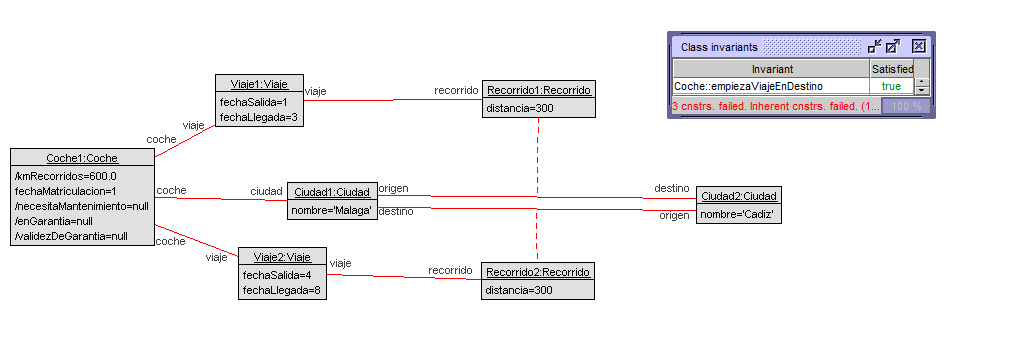
\includegraphics[width=1\linewidth]{Soils/10.png}
     \caption{Diagrama de objetos para la invariante al cumplirse}
     \label{Diagrama del sistema de aviacion}
\end{figure}

\begin{figure}[H]
     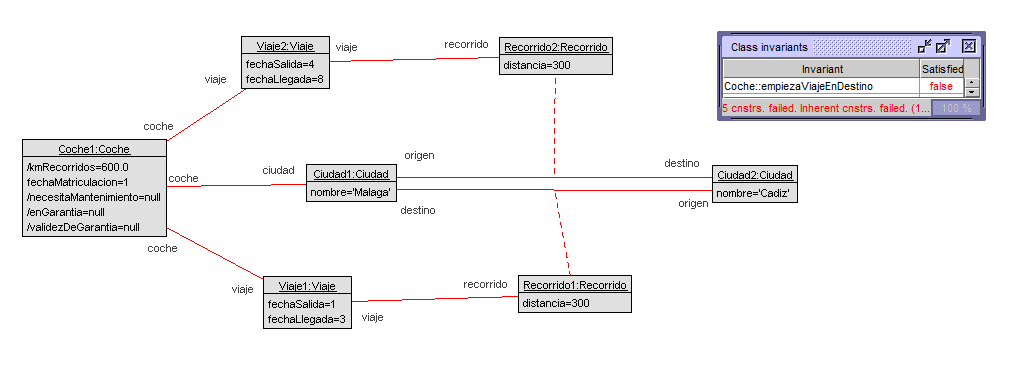
\includegraphics[width=1\linewidth]{Soils/10_v2.png}
     \caption{Diagrama de objetos para la invariante al incumplirse}
     \label{Diagrama del sistema de aviacion}
\end{figure}

La invariante 10 establece que un coche debe encontrarse en la ciudad destino de su último viaje antes de iniciar uno nuevo. Se cumple cuando el coche está en la ciudad de destino de su último viaje. No se cumple si el coche no está en esta ciudad antes de iniciar un nuevo viaje.

\subsubsection{Invariante 11: viajeDespuesdeMatriculacion}
    \begin{figure}[H]
         \centering
         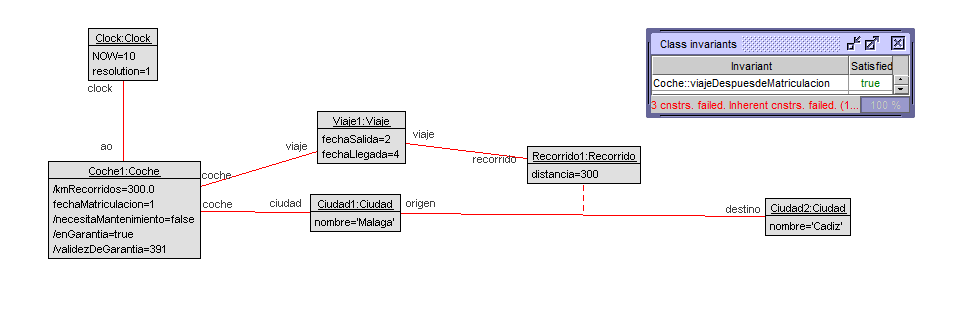
\includegraphics[width=1\linewidth]{Soils/11.png}
         \caption{Diagrama de objetos para la invariante al cumplirse}
         \label{Diagrama_cumplimiento}
    \end{figure}

    
 \begin{figure}[H]
    \centering
    \begin{minipage}{0.49\textwidth}
        \centering
        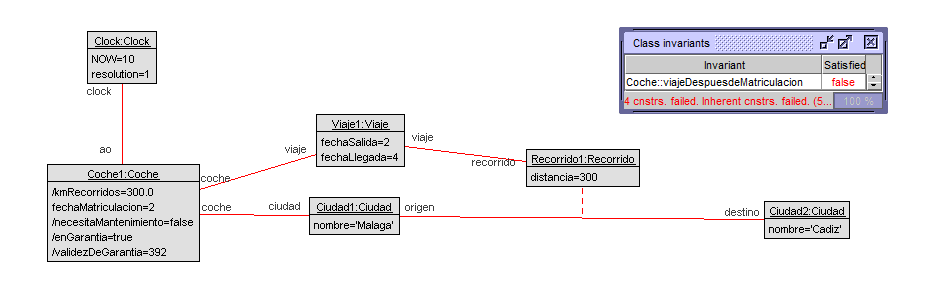
\includegraphics[width=1\linewidth]{Soils/11_v2.png}
        \label{fig:diagrama1}
    \end{minipage}
    \hfill
    \begin{minipage}{0.49\textwidth}
        \centering
        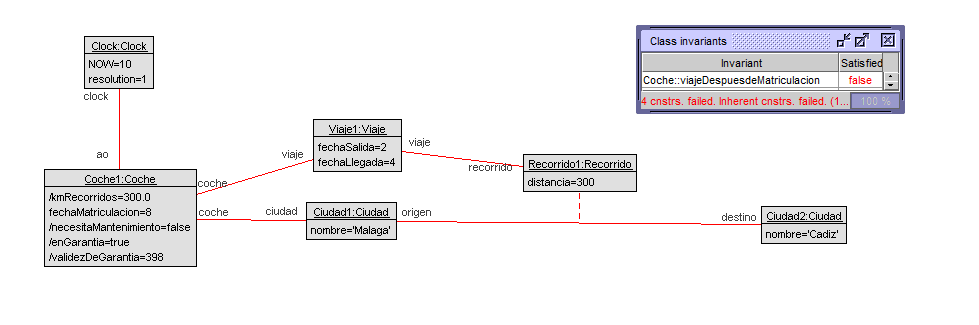
\includegraphics[width=1\linewidth]{Soils/11_v3.png}
        \label{fig:diagrama2}
    \end{minipage}
    \caption{Diagramas de objetos para la invariante al incumplirse}
    \label{fig:diagrama_invariante}
\end{figure}

La invariante 11 prohíbe que un coche viaje antes de su fecha de matriculación. Se cumple cuando el coche viaja después de la fecha de matriculación. No se cumple si el viaje se realiza antes de esa fecha.

\subsubsection{Invariante 12: noViajeEnMantenimiento}

\vspace{1.0 cm}
\begin{figure}[H]
     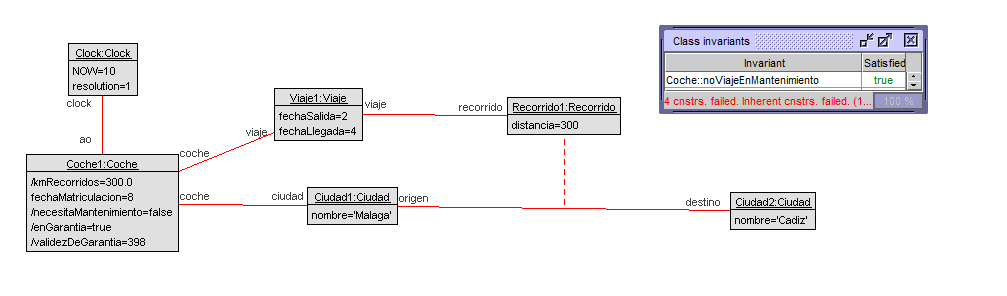
\includegraphics[width=1\linewidth]{Soils/12.png}
     \caption{Diagrama de objetos para la invariante al cumplirse}
     \label{Diagrama del sistema de aviacion}
\end{figure}

\begin{figure}[H]
     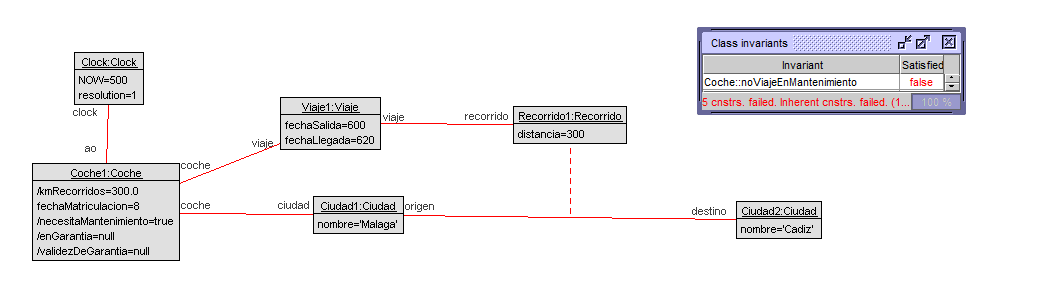
\includegraphics[width=1\linewidth]{Soils/12_v2.png}
     \caption{Diagrama de objetos para la invariante al incumplirse}
     \label{Diagrama del sistema de aviacion}
\end{figure}

La invariante 12 asegura que un coche no puede comenzar un viaje con la flag de necesitaMantenimiento activa. Se cumple cuando el coche no tiene la alerta de mantenimiento activa al iniciar un viaje. No se cumple si el coche inicia un viaje con la alerta de mantenimiento en true.

\subsubsection{Invariante 13: fechaViajeBienDefinida}
\begin{figure}[H]
        \begin{minipage}{0.49\textwidth}
            \centering
            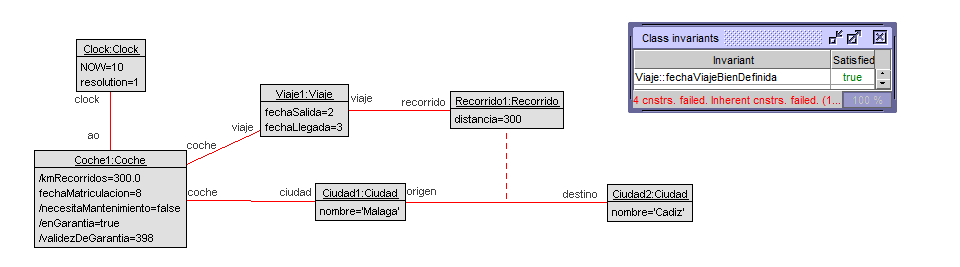
\includegraphics[width=1\linewidth]{Soils/13.png}
        \end{minipage}
        \hfill
        \begin{minipage}{0.49\textwidth}
        \centering
        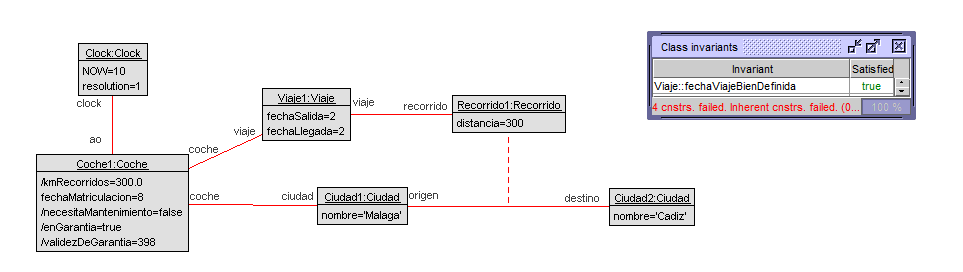
\includegraphics[width=1\linewidth]{Soils/13_v2.png}
        \label{fig:diagrama2}
    \end{minipage}
            \caption{Diagrama de objetos para la invariante al cumplirse}
         \label{Diagrama_cumplimiento}
\end{figure}

    
 \begin{figure}[H]
     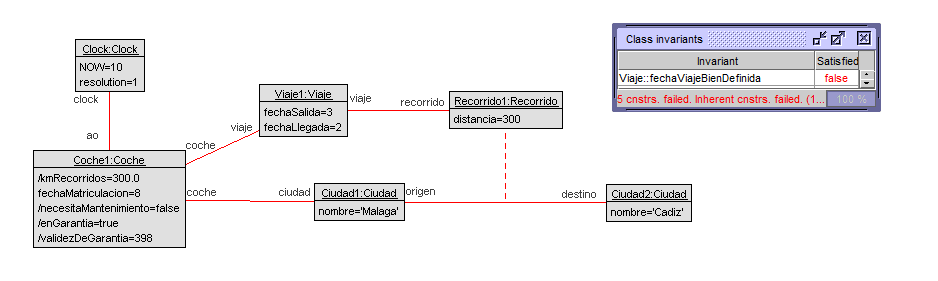
\includegraphics[width=1\linewidth]{Soils/13_v3.png}
     \caption{Diagrama de objetos para la invariante al incumplirse}
     \label{Diagrama del sistema de aviacion}
\end{figure}

La invariante 13 establece que un viaje no puede tener una fecha de inicio posterior a su fecha de llegada. Se cumple cuando la fecha de inicio es anterior o igual a la fecha de llegada. No se cumple si la fecha de inicio es posterior a la de llegada.\\\\
De esta manera podemos comprobar que todas las restricciones se cumplen.

\newpage
\section{Modelado Dinámico}
En este apartado, se debe entregar la imagen del diagrama de clases y el código USE desarrollado (al ser este apartado un incremento respecto del anterior, hay que entregar únicamente el código USE nuevo). En las operaciones añadidas, especificar las pre- y post- condiciones.

\subsection{Diagrama de clases}
\begin{figure}[H]
     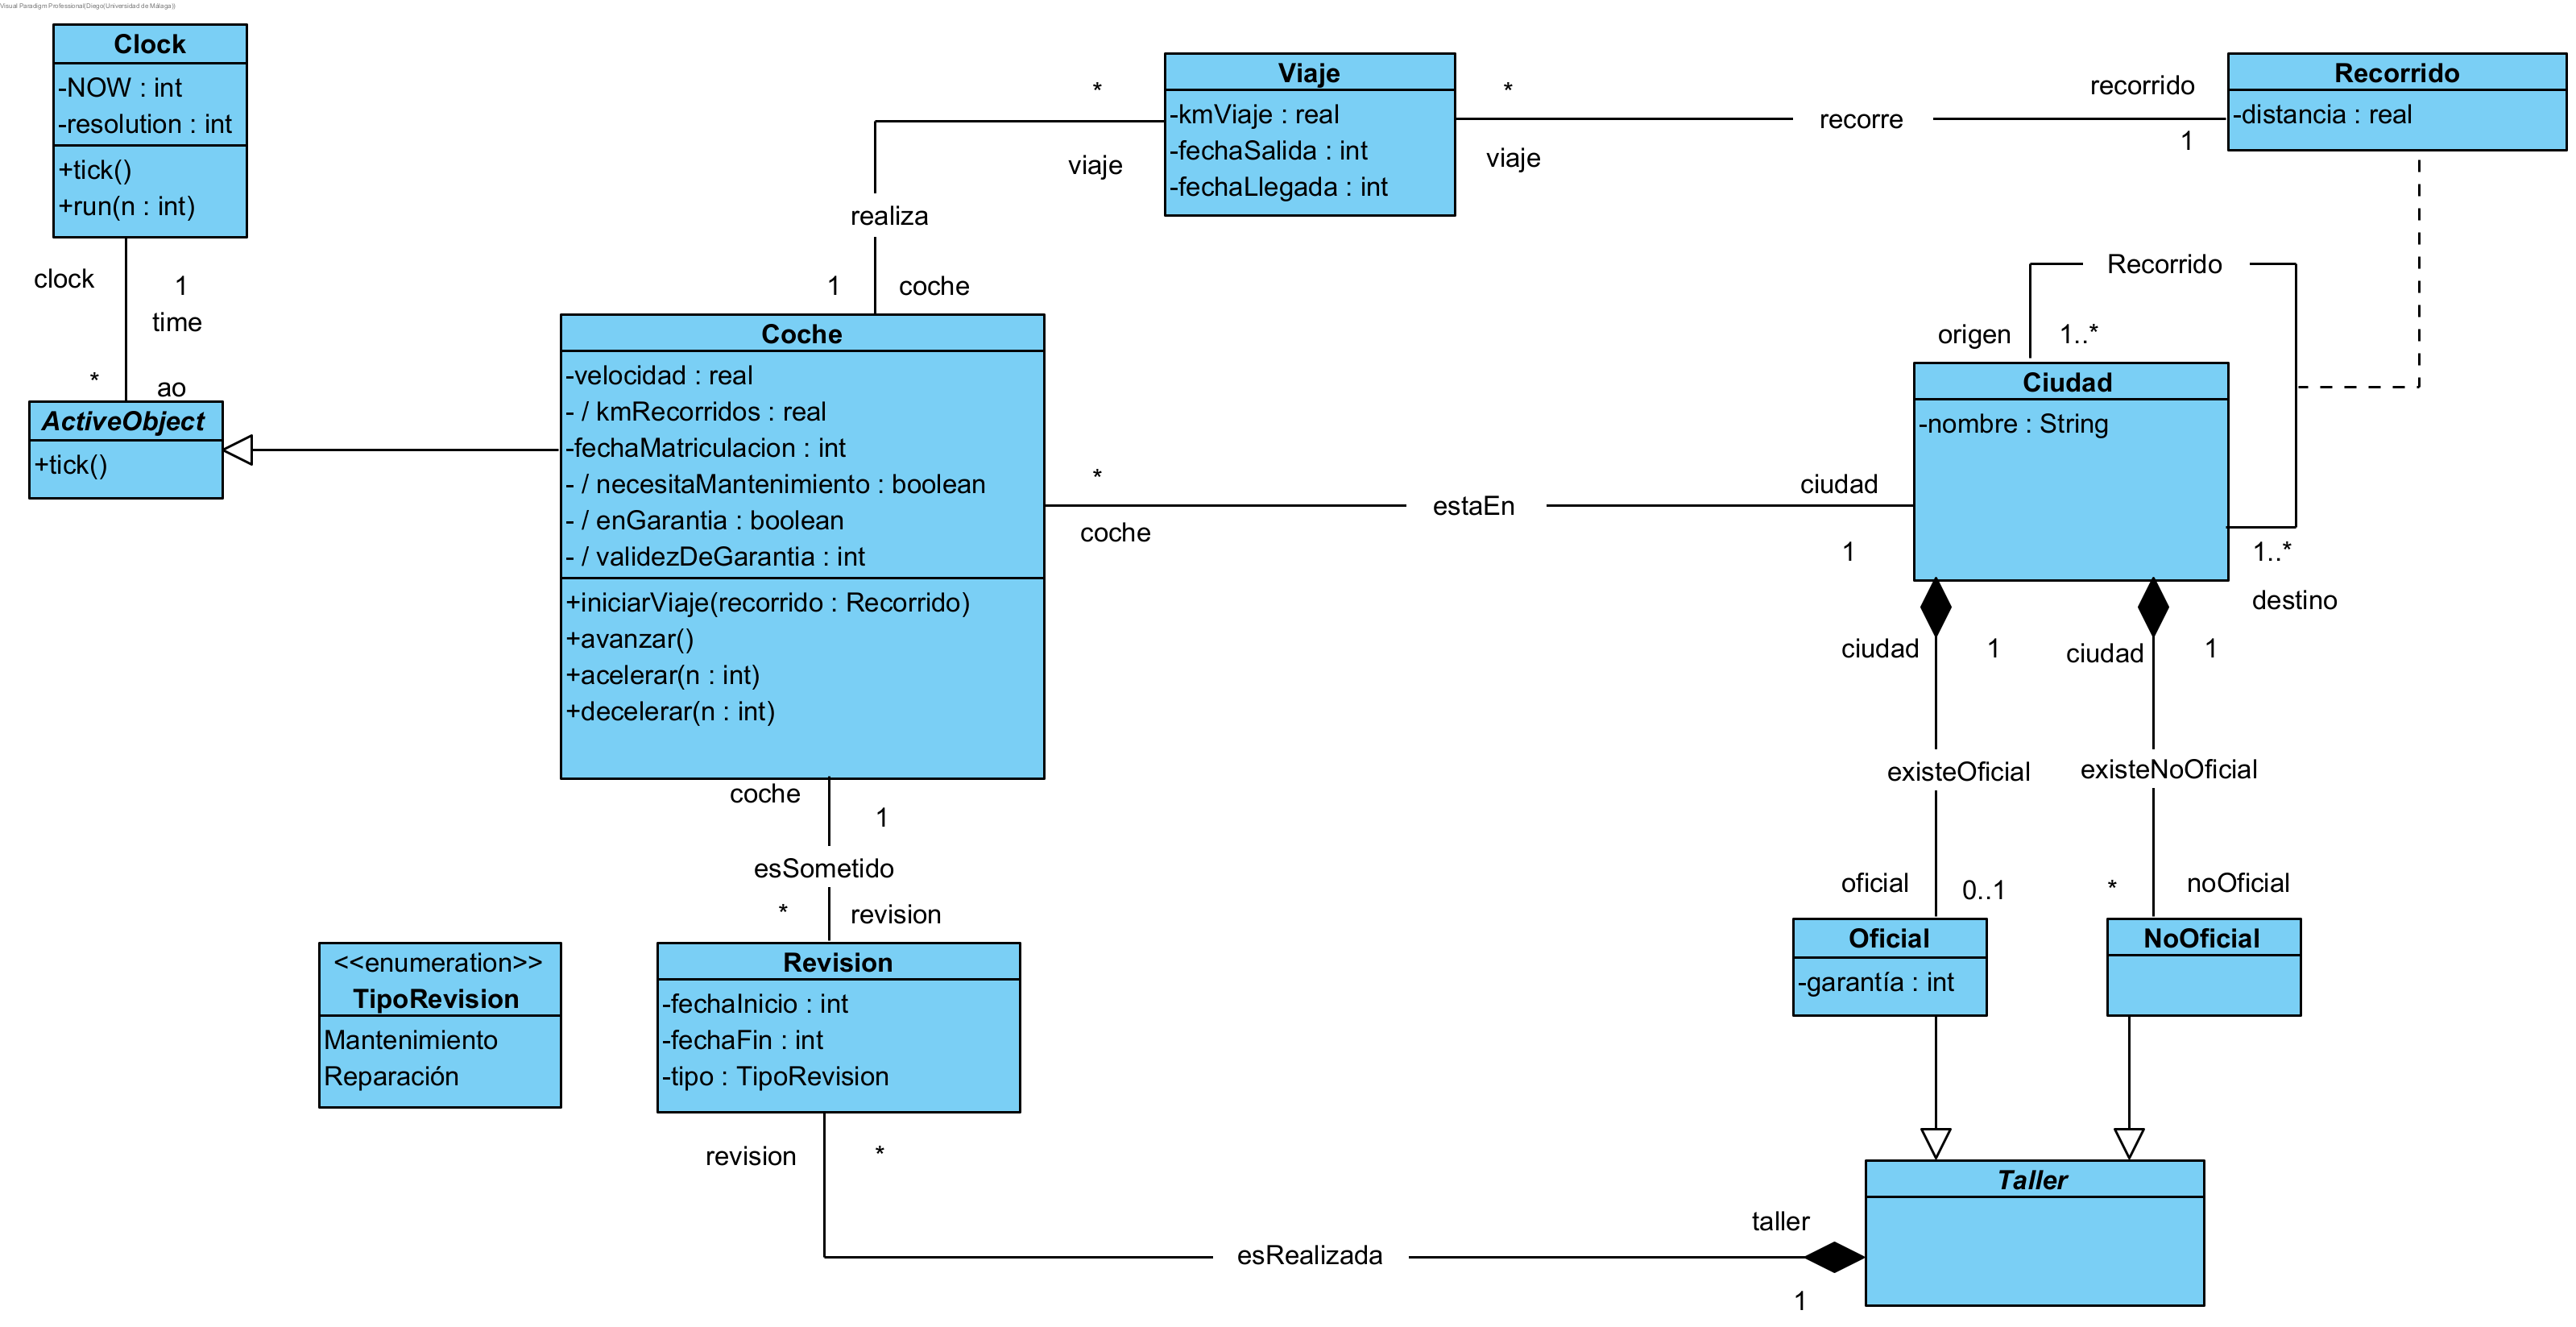
\includegraphics[width=1\linewidth]{diagramas/VPP_B.png}
     \caption{Diagrama del sistema de coches para el modelo dinámico}
     \label{Diagrama del sistema de coches}
\end{figure}

A diferencia del diagrama del modelo estructural, en este modelo hemos añadido dos atributos nuevos en las clases Coche y Viaje. Con estos atributos adicionales, el modelo puede ofrecer una representación más completa y precisa de los trayectos y los coches involucrados.

\subsection{Novedades y modificaciones en las clases del sistema dinámico}
\subsubsection{Clock}
\textbf{Descripción}:  Hemos añadido las operaciones tick() y run(n:Integer) para simular el paso del tiempo.
\begin{itemize}
    \item \textbf{Operaciones:}
    \begin{itemize}
        \item \texttt{tick()}: Usada para avanzar en el tiempo la cantidad definida en \emph{resolution}.
        \item \texttt{run(n : Integer)}: Permite avanzar en el tiempo \emph{n} pasos en un solo tick.
    \end{itemize}
\end{itemize}
    
\subsubsection{ActiveObject}
\textbf{Descripción}:  Hemos añadido la operación tick() para que los objetos que hereden de la clase ActiveObject se vean afectados por el paso del tiempo.
\begin{itemize}
    \item \textbf{Operaciones:}
    \begin{itemize}
        \item \texttt{tick()}: Invoca el método tick() de la instancia de Clock. Esto significa que cada objeto activo tiene acceso a la funcionalidad del reloj y puede actualizar el tiempo del sistema llamando al método tick() de Clock.
    \end{itemize}
\end{itemize}

\subsubsection{Coche}
\textbf{Descripción}:  Hemos añadido el atributo "velocidad" que en un inicio vale 0 como también varias operaciones como iniciarViaje(recorrido : Recorrido), avanzar(), acelerar(n : Integer), decelerar(n : Integer) y tick().
\begin{itemize}
    \item \textbf{Atributos:}
    \begin{itemize}
        \item \texttt{velocidad: Real init : 0 }: Velocidad del coche. Inicialmente está en 0, es decir, que está parado.
        \item \texttt{kmRecorridos: Real (derive)}: En el dinámico consideramos que si existen viajes previos, el cálculo se realiza sumando las distancias de los recorridos de todos los viajes anteriores, excluyendo el último viaje. A este valor se le añade el kilometraje del último viaje (kmViaje) para obtener el total de kilómetros recorridos por el coche. Esto permite tener un registro dinámico y actualizado de la distancia total recorrida por el coche a medida que se realizan nuevos viajes.
    \end{itemize}
    \item \textbf{Operaciones:}
    \begin{itemize}
        \item \texttt{iniciarViaje(recorrido : Recorrido)}: Esta operación inicia un nuevo viaje para el coche. Se crea un objeto Viaje, se establece la fecha de salida como el tiempo actual y se relaciona al coche con el viaje y el recorrido correspondiente. También actualiza la ciudad en la que se encuentra el coche, eliminándola de la relación estaEn.
        \item \texttt{avanzar())}: Esta operación actualiza el kilometraje del coche durante su viaje, sumando su velocidad actual al kilometraje recorrido. Si el coche ha alcanzado la distancia total del recorrido, la operación finaliza el viaje, marca la fecha de llegada y actualiza la ciudad en la que el coche termina su viaje.
        \item \texttt{acelerar(n : Integer)}: Permite incrementar la velocidad del coche en n unidades. La operación ajusta la velocidad del coche sumando el valor n a la velocidad actual.
        \item \texttt{decelerar(n : Integer)}: Reduce la velocidad del coche en n unidades, siempre que la velocidad actual sea mayor o igual al valor n. Esto disminuye la velocidad del coche de acuerdo al valor especificado.
        \item \texttt{tick()}: Actualiza el estado del coche en función del tiempo. Si el coche está en un viaje en curso, avanza en su trayecto según la velocidad y distancia recorrida. Esta operación depende del reloj del sistema para actualizar el tiempo y garantizar el progreso del coche en su viaje.
    \end{itemize}
\end{itemize}


\subsubsection{Coche}
\textbf{Descripción}:  Hemos añadido el atributo "kmViaje" que en un inicio vale 0.
\begin{itemize}
    \item \textbf{Atributos:}
    \begin{itemize}
        \item \texttt{kmViaje : Real init : 0 }: Los kilómetros que ha realizado el coche durante el viaje.
    \end{itemize}
\end{itemize}

\subsection{Diagrama de Clases del modelo dinámico en USE}
La herramienta USE nos permite llevar a cabo un diagrama de clases para el modelo dinámico, el cual se muestra a continuación:
\begin{figure}[H]
     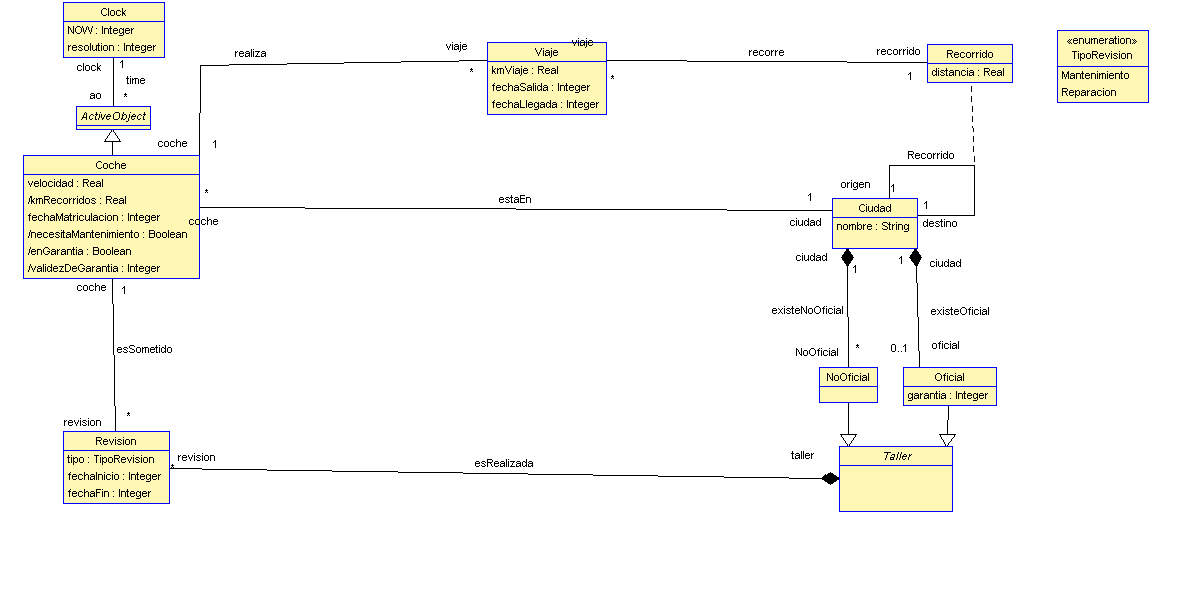
\includegraphics[width=1\linewidth]{diagramas/USE_B.png}
     \caption{Diagrama del sistema de coches en USE}
     \label{Diagrama del sistema de coches en USE}
\end{figure}

Las relaciones en el modelo dinámico se mantienen igual que en el modelo estructural que ya se han descrito anteriormente.


\subsection{Modificaciones de las invariantes en el modelo dinámico}
\subsubsection{Inv4: Si un coche está en revisión, debe de estar en la misma ciudad que el taller}
    \begin{lstlisting}[style = useEspecifico,language=SQL]
context Revision
    inv mismaCiudadqueTallerEnRevision :
    self.fechaFin = null implies 
    (self.taller.oclIsKindOf(Oficial) and self.taller.oclAsType(Oficial).ciudad = self.coche.ciudad)
    or
    (self.taller.oclIsKindOf(NoOficial) and self.taller.oclAsType(NoOficial).ciudad = self.coche.ciudad)
    \end{lstlisting}
    Es una modificacioón con respecto al modelo estático ya que en dicho modelo se comparaba el tiempo del clock con la fecha final ya que al ser estático estaba prefijada antes de empezar la revisión, y en el dinámico tenemos la fecha de final a null mientras este en la revisión con eso podemos comprobar si esta en un taller o no y ya con dicha información sabemos si se encuentran en la misma ciudad.

\subsubsection{Inv5: Un coche tiene que estar o viajando o en una ciudad}
    \begin{lstlisting}[style = useEspecifico,language=SQL]
context Viaje
    inv viajandoOenCiudad:
    self.fechaLlegada = null implies
    self.coche.ciudad.oclIsUndefined() and self.coche.estaEn->notEmpty()
    \end{lstlisting}
    Es una modificación con respecto al modelo estático ya que en dicho modelo se comparaba el tiempo del clock con la fecha final ya que al ser estático estaba prefijada antes de empezar el viaje, mientras que en el dinámico la fecha de llegada es null ya que esta de viaje, y esta es igual al tiempo del clock cuando ha terminado dicho recorrido.


\subsubsection{Inv13: Un viaje no puede tener una fecha de inicio superior a su fecha de llegada}
    \begin{lstlisting}[style = useEspecifico,language=SQL]
context Viaje
    inv fechaViajeBienDefinida:
    (self.fechaLlegada <> null) or (self.fechaLlegada >= self.fechaSalida)
    \end{lstlisting}
    En esta invariante añadimos la primera parte del or con el null para ya que al estar en el viaje dicho atributo se encuentra en null por lo que si no lo añadieramos daría fallo el modelo.

\subsection{Añadimos soils???}
    
\subsection{b3}
Un coche comienza un viaje desde la ciudad en la que se encuentra. Esta operación debe recibir como parámetro el recorrido entre dos ciudades que debe realizar en su viaje.
Una operación avanzar que se ejecuta sobre los coches, y que no recibe ningún parámetro. Esta operación debe hacer avanzar el coche el número de kilómetros indicados en su velocidad si el coche está realizando algún viaje. Se debe modelar el paso del tiempo, de modo que un tic del reloj representa el paso de un día, lo cual se debe tener en cuenta a la hora de que los coches puedan avanzar en el viaje que estén realizando.

\newpage
\section{Caso Particular}
Ahora se debe desarrollar un modelo de objetos y simularlo. Vamos a considerar tres ciudades: Málaga, Sevilla y Granada. Tendremos dos recorridos: entre Málaga y Sevilla con 210 kilómetros, y entre Sevilla y Granada con 250 kilómetros. Supondremos un coche matriculado en el instante 0 (día 0) y que viaja a una velocidad de 27. El coche comienza en Málaga y continúa en Málaga hasta el día 5, día en que comienza un viaje haciendo el recorrido de Málaga a Sevilla. Los días van pasando y el coche va avanzando hasta que llega a Sevilla. El mismo día que llega a Sevilla, el coche comienza otro viaje haciendo el recorrido entre Sevilla y Granada. Los días van pasando y el coche continúa realizando el viaje. Una vez llega a Granada, la simulación termina.
Se debe mostrar 3 imágenes del diagrama conceptual: una en el instante 0, otra cuando el coche llega a Sevilla y otra cuando el coche lleva a Granada. Entregar también el código SOIL necesario para reproducir el modelo conceptual y la simulación.


\newpage
\section{Conclusión}
\lipsum[]


\end{document}
